% %set_parent(‘/Users/mwilli/Documents/Spring_2017/Dissertation_Document/Dissertation_Working_Directory_Draft/Dissertation_Main.Rnw')
% 
% <<chunk_options, echo=FALSE>>=
% # This is where we set basic knitr options.
% opts_chunk$set(echo=TRUE, message=FALSE, warning = FALSE, cache = FALSE, comment="")
% options(width=75) # This sets how wide the R printout can be.
% @
% 
%  <<setup-child, include=FALSE>>=
%  set_parent('/home/sam/Dissertation/Dissertation_Template/Dissertation_Main_Template/Dissertation_Main.Rnw')
% @
% 
% <<load_libraries, echo=FALSE>>=
% library(tidyr)
% library(dplyr)
% library(ggplot2)
% library(lme4)
% library(lsmeans)
% library(car)
% library(pbkrtest)
% library(xtable)
% library(cowplot)
% library(plyr)
% @

\chapter{Introduction\label{chapter1}}

Speech in a noisy background presents a challenge for recognition of that speech both by human listeners and by computers tasked with understanding human speech (automatic speech recognition; ASR).  Years of research have resulted in a variety of solutions, that have not completely solved the problem.  Most approaches have taken the route of trying to remove noise from a signal that is already corrupted with noise.

Figure \ref{fig:signal-SNR-intro} demonstrates this problem.  The dark horizontal bands seen in the spectrogram in each subfigure are part of the speech signal.  In Figure \ref{fig:signal-SNR-intro-low}, these are clearly visible above the background noise.  By contrast, in Figure \ref{fig:signal-SNR-intro-high}, these dark horizontal bands are more difficult to see.  The amplitude (level of darkness in the spectrogram) of the noise at various frequencies drowns out the speech signal, making it more difficult to hear.  In the noisy signal, there is more competing information that makes it difficult for both humans - and computers - to differentiate what is noise and what is speech.  This will be discussed in more depth in Section \ref{sec:snr-difficult}.

This project presents a new approach to the problem.  It proposes that human speech can be recorded in a manner that largely eliminates the noise before it reaches the microphone recording the signal.  The microphone would be placed inside the ear canal of the speaker and would record speech as it is passed through the bone and tissue of the speaker's head.  The signal is expected to be distorted by passage through the head, but the speech is expected to be recoverable.  This has potential wide-ranging applications, including human-to-human electronic communication in loud workplaces (eg. factory floor, airport tarmac), as well as human-to-computer interactions, as the use of artificial intelligence becomes more widespread and mainstream; this includes its use in such noisy workplace environments.

\begin{figure}[H]
\centering
\begin{subfigure}{\textwidth}
\centering
  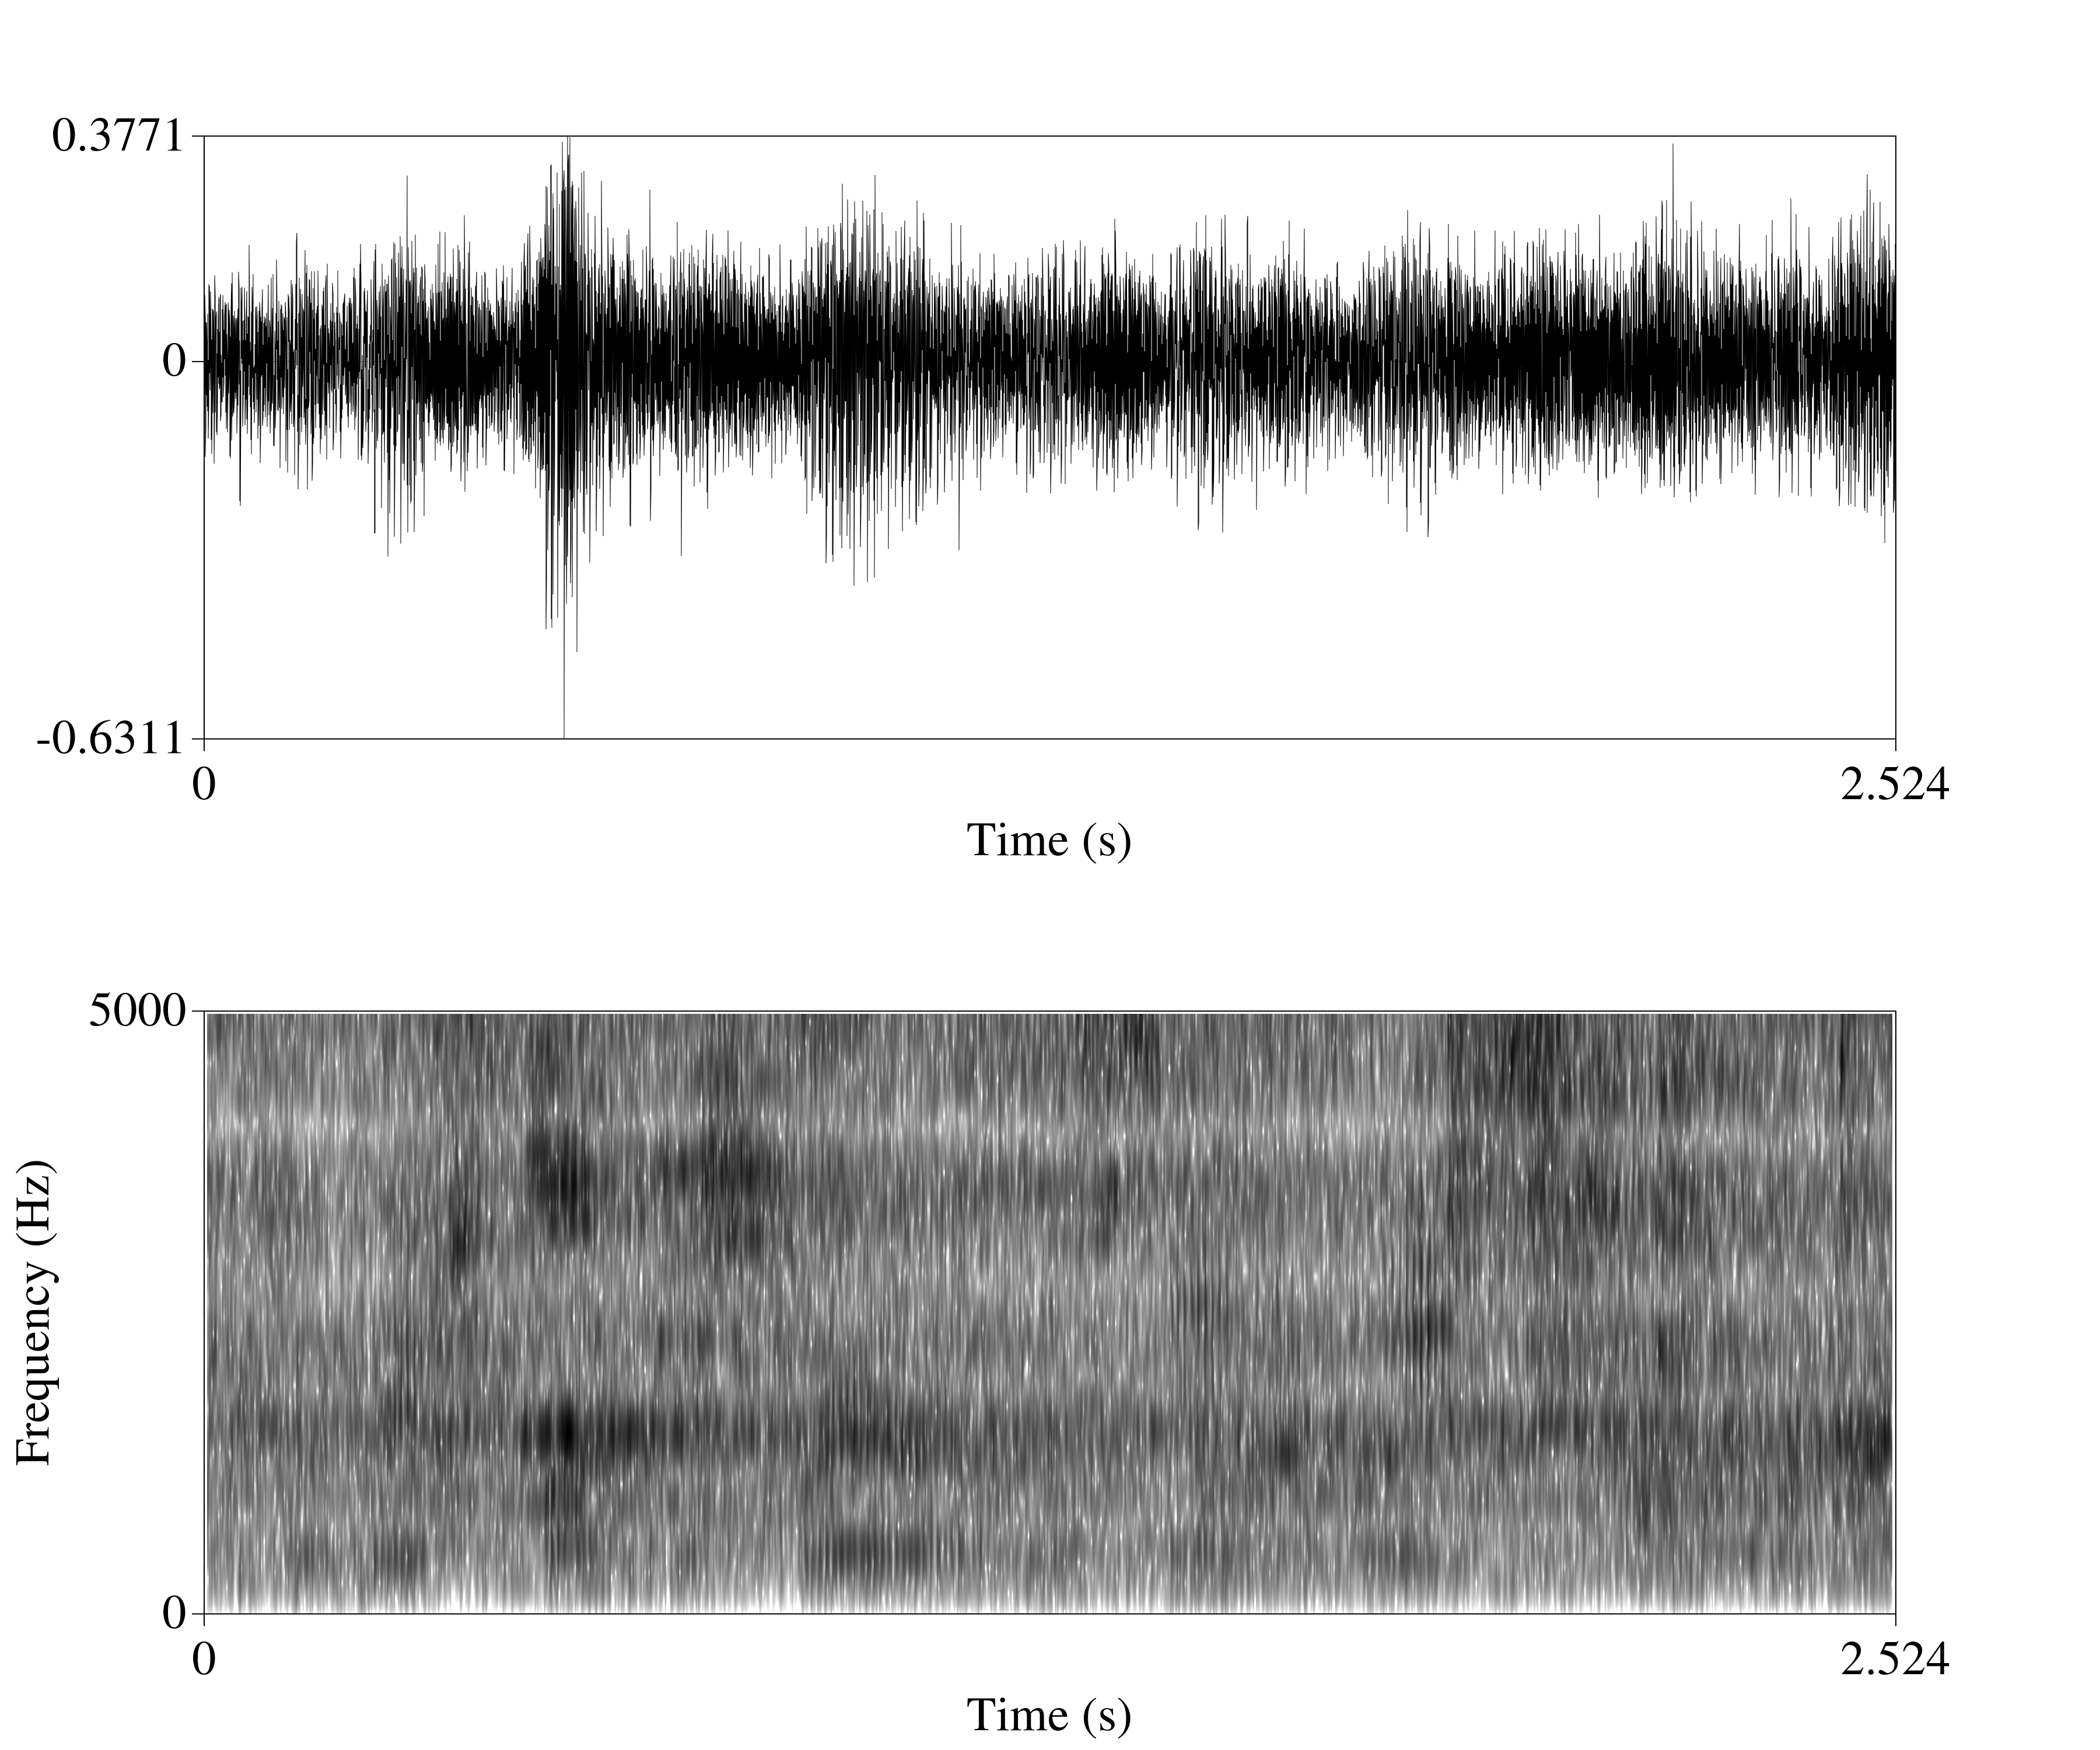
\includegraphics[width=.8\textwidth]{figure/signal-SNR-intro-low.png}
  \caption{A sentence spoken with a low level of background noise, resulting in a \textit{high} SNR.}
  \label{fig:signal-SNR-intro-high}
\end{subfigure}
%
\begin{subfigure}{\textwidth}
\centering
  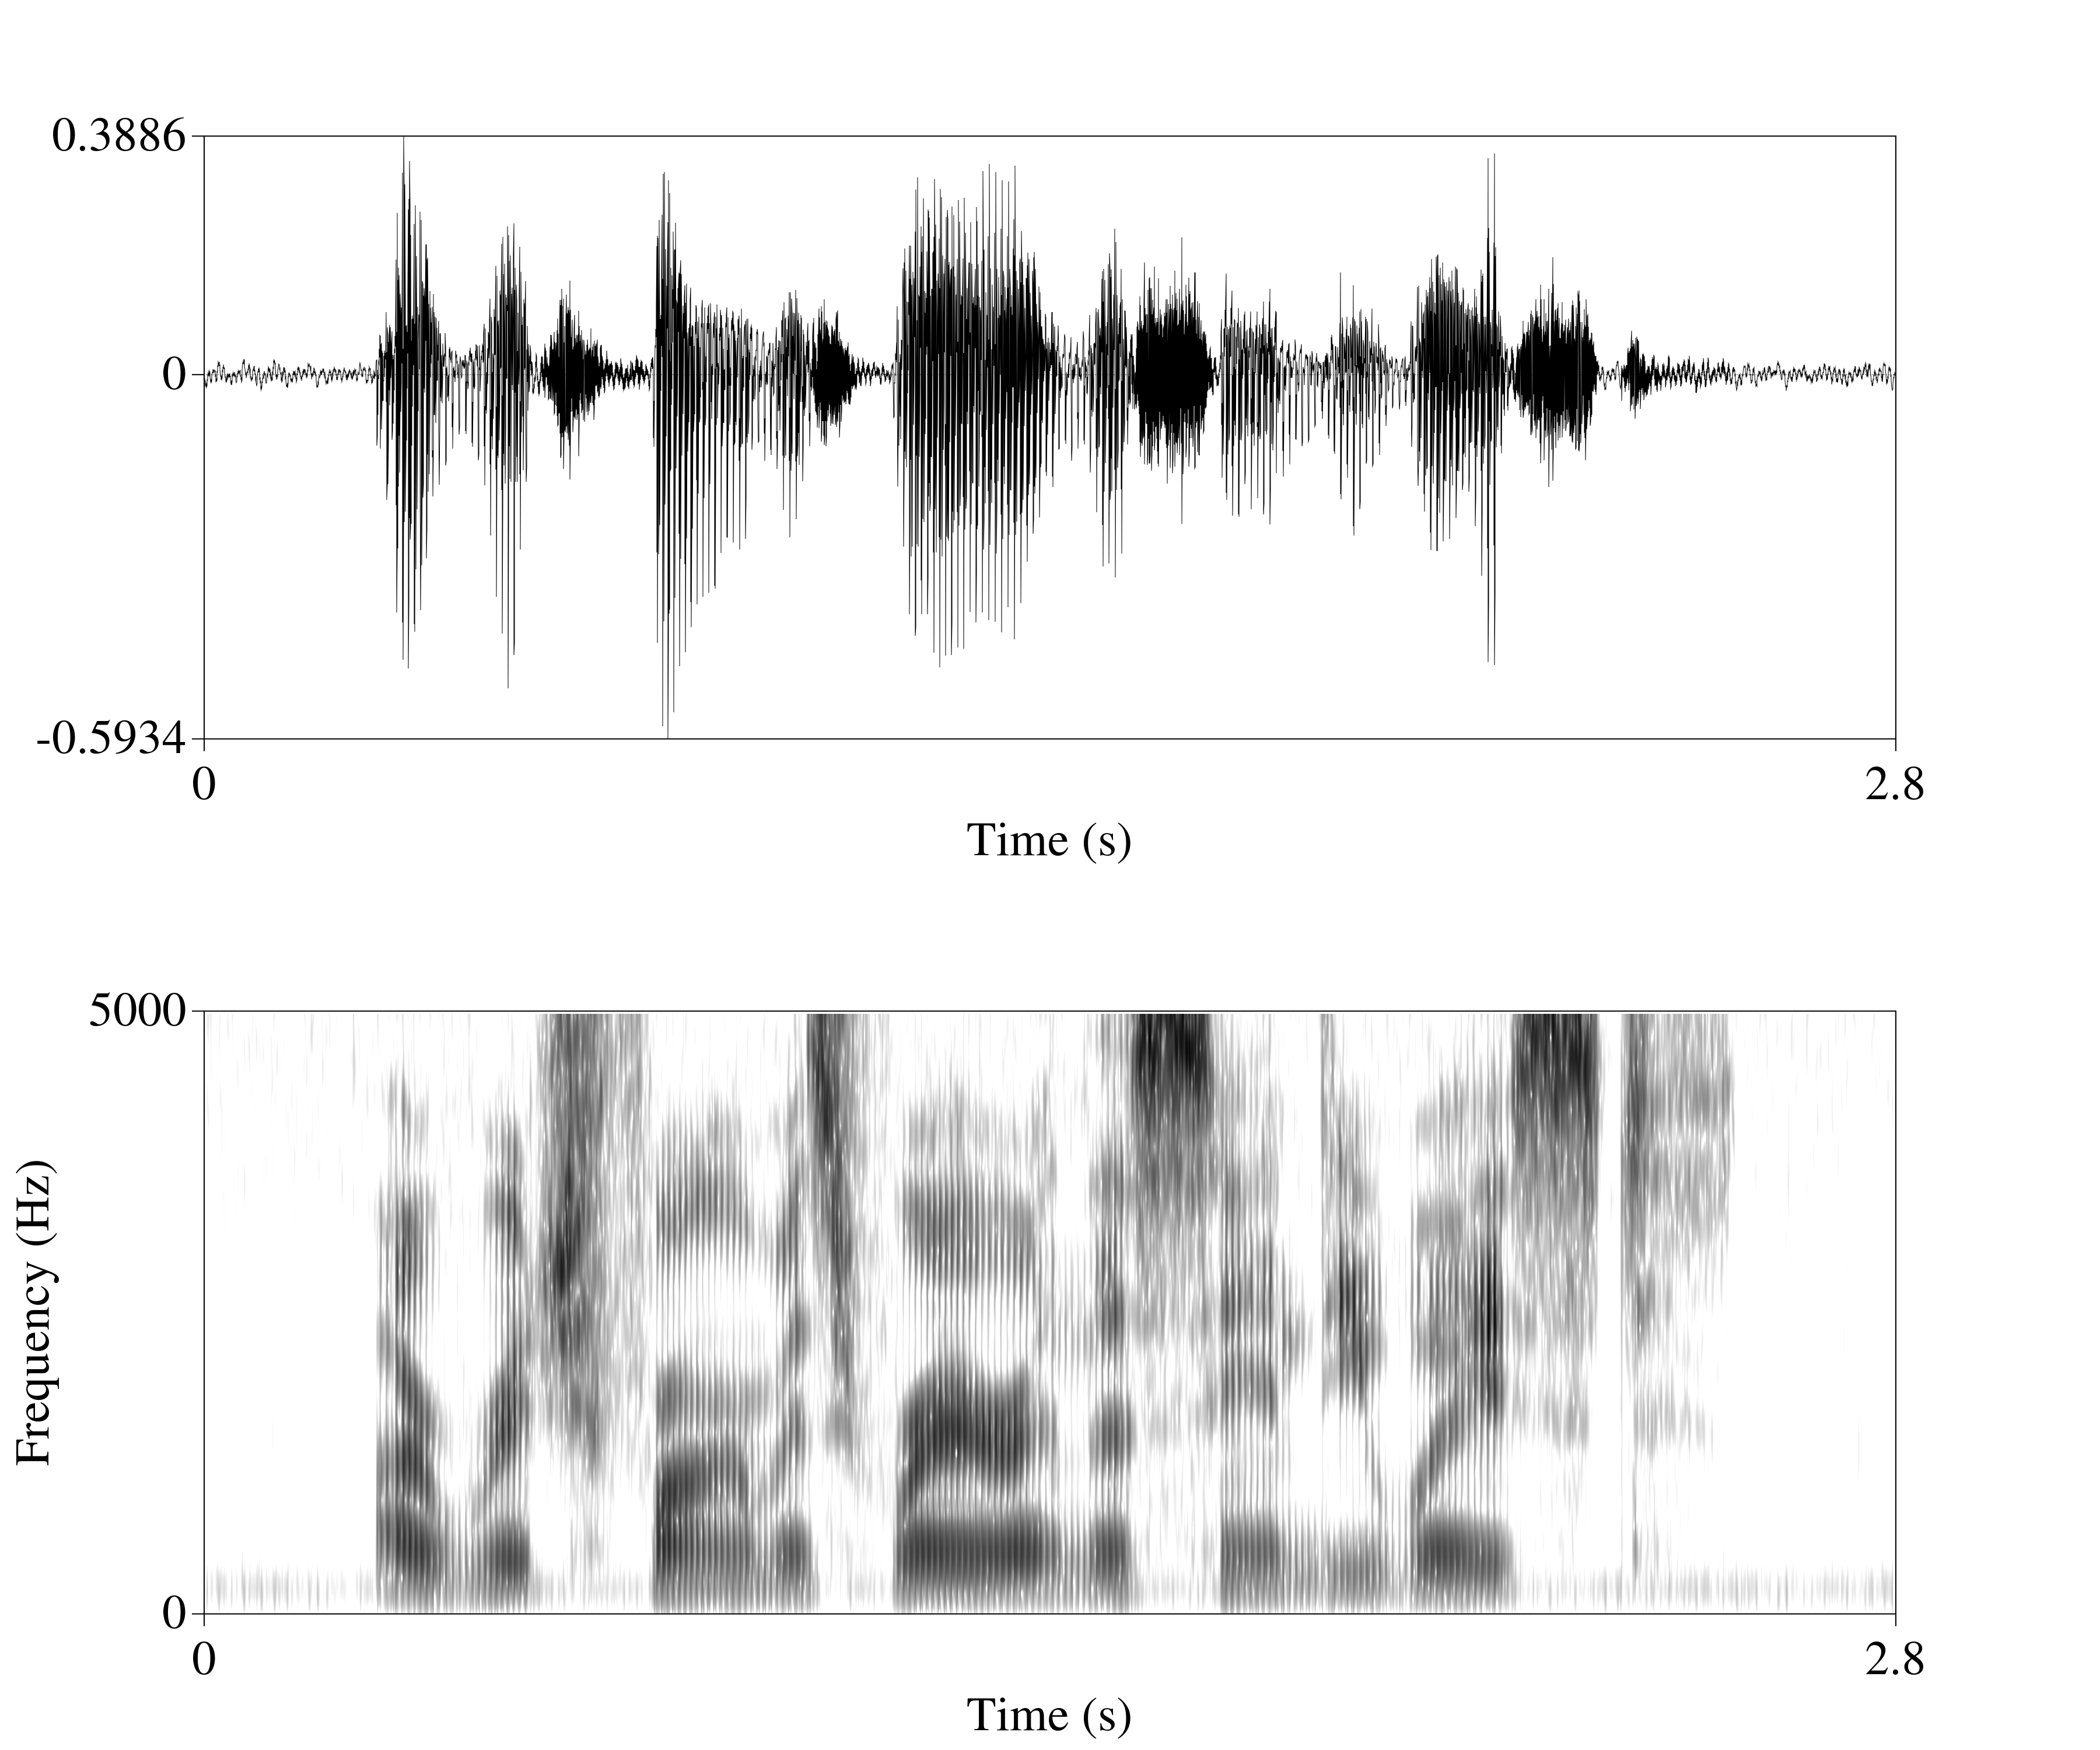
\includegraphics[width=.8\textwidth]{figure/signal-SNR-intro-high.png}
  \caption{A sentence spoken with a high level of background noise, resulting in a \textit{low} SNR.}
  \label{fig:signal-SNR-intro-low}
\end{subfigure}
\caption{Waveforms and spectrograms of the sentence ``The glow deepened in the eyes of the sweet girl.''}
\label{fig:signal-SNR-intro}
\end{figure}

Section \ref{ch1:background} below describes the basic acoustics of sound.  This is intended to be a general background to acoustics and interfering sound waves, leading up to a brief overview of sound in noise. Chapter \ref{chapter2} discusses the collection of ear-recorded speech, Chapter \ref{chapter3} describes a human speech perception experiment using ear-recorded speech, and Chapter \ref{chapter4} outlines an experiment testing the ability of an automatic speech recognition system to accurately recognize ear-recorded speech.  At the end of this chapter, Section \ref{ch1:diss-overview} gives a more detailed overview of the rest of the dissertation.

\section{Background}\label{ch1:background}

Sound itself, along with the ability to perceive it, is a remarkable phenomenon.  Put simply, `sound' is the fluctuation of pressure in neighboring groups of particles over time. Most frequently sound is discussed in terms of the fluctuation of air pressure, because, as humans, we primarily receive sound into our ear canals through the medium of air, but sound can also travel through liquids and solids, or pass through any combination of the three.

There are primarily three components to sound: amplitude, frequency, and phase (\cite{rosen:91}), which can be seen in Figure \ref{fig:basic-sound-wave}.  In a simple sound wave, the amplitude of sound corresponds to the peak intensity of the high pressure (and the lowest pressure) portions of a sound wave (cf. Fig. \ref{fig:basic-sound-amplitude}).  The frequency corresponds to the rate at which the high and low pressure portions of the signal fluctuate between one another (cf. Fig. \ref{fig:basic-sound-frequency}).  The phase of a wave is the location of the pressure level (relative to atmospheric pressure) at a given moment in time (cf. Fig. \ref{fig:basic-sound-phase}).

This latter characteristic - phase, while important when dealing with interacting waves from multiple sources, is often not taken into account in speech science due to both its complexity and the fact that phase does not encode critical speech information.  The human auditory system primarily makes use of the other two characteristics of sound - amplitude and frequency.

\begin{figure}[H]
\begin{subfigure}{0.5\textwidth}
  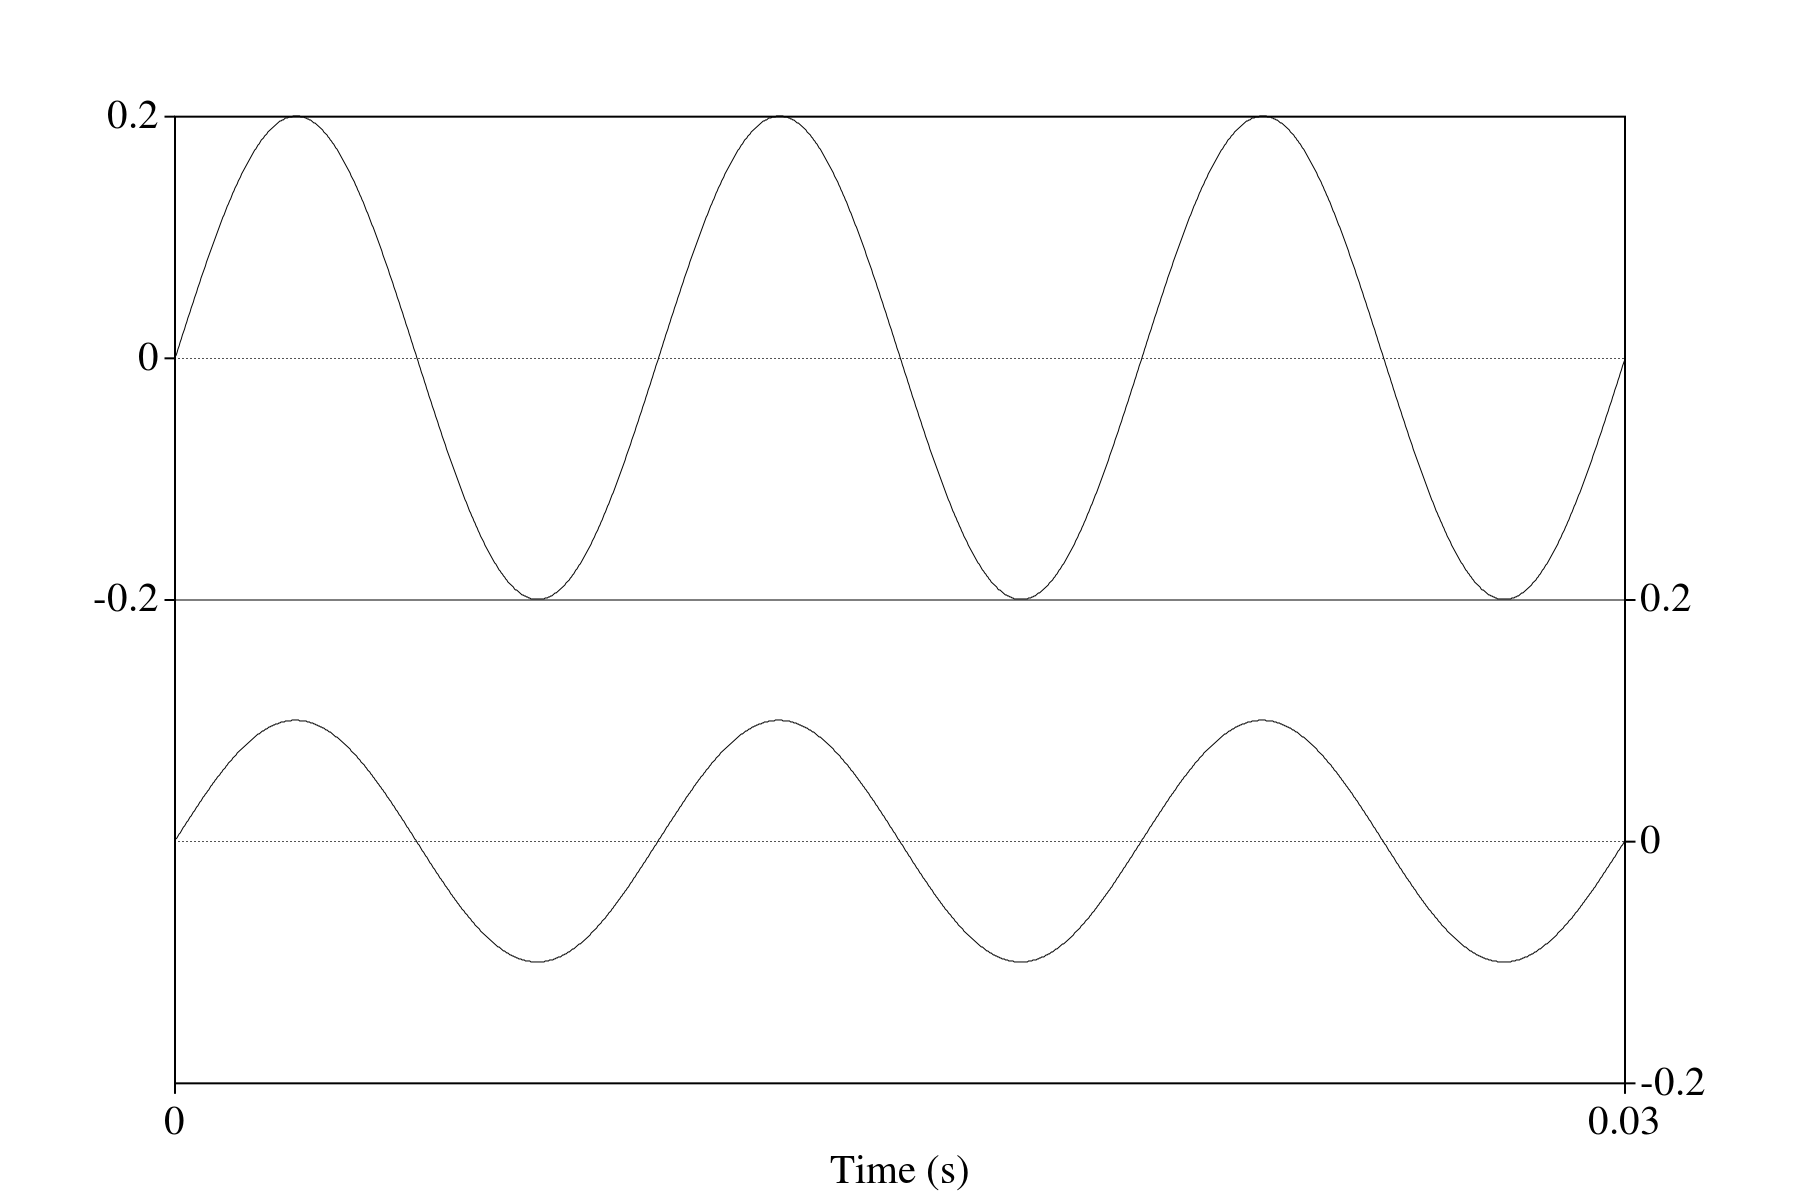
\includegraphics[width=\textwidth]{figure/basic-sound-amplitude.png}
  \caption{Two waveforms showing a difference in amplitude between the two signals.}
  \label{fig:basic-sound-amplitude}
\end{subfigure}
\qquad
\begin{subfigure}{0.5\textwidth}
  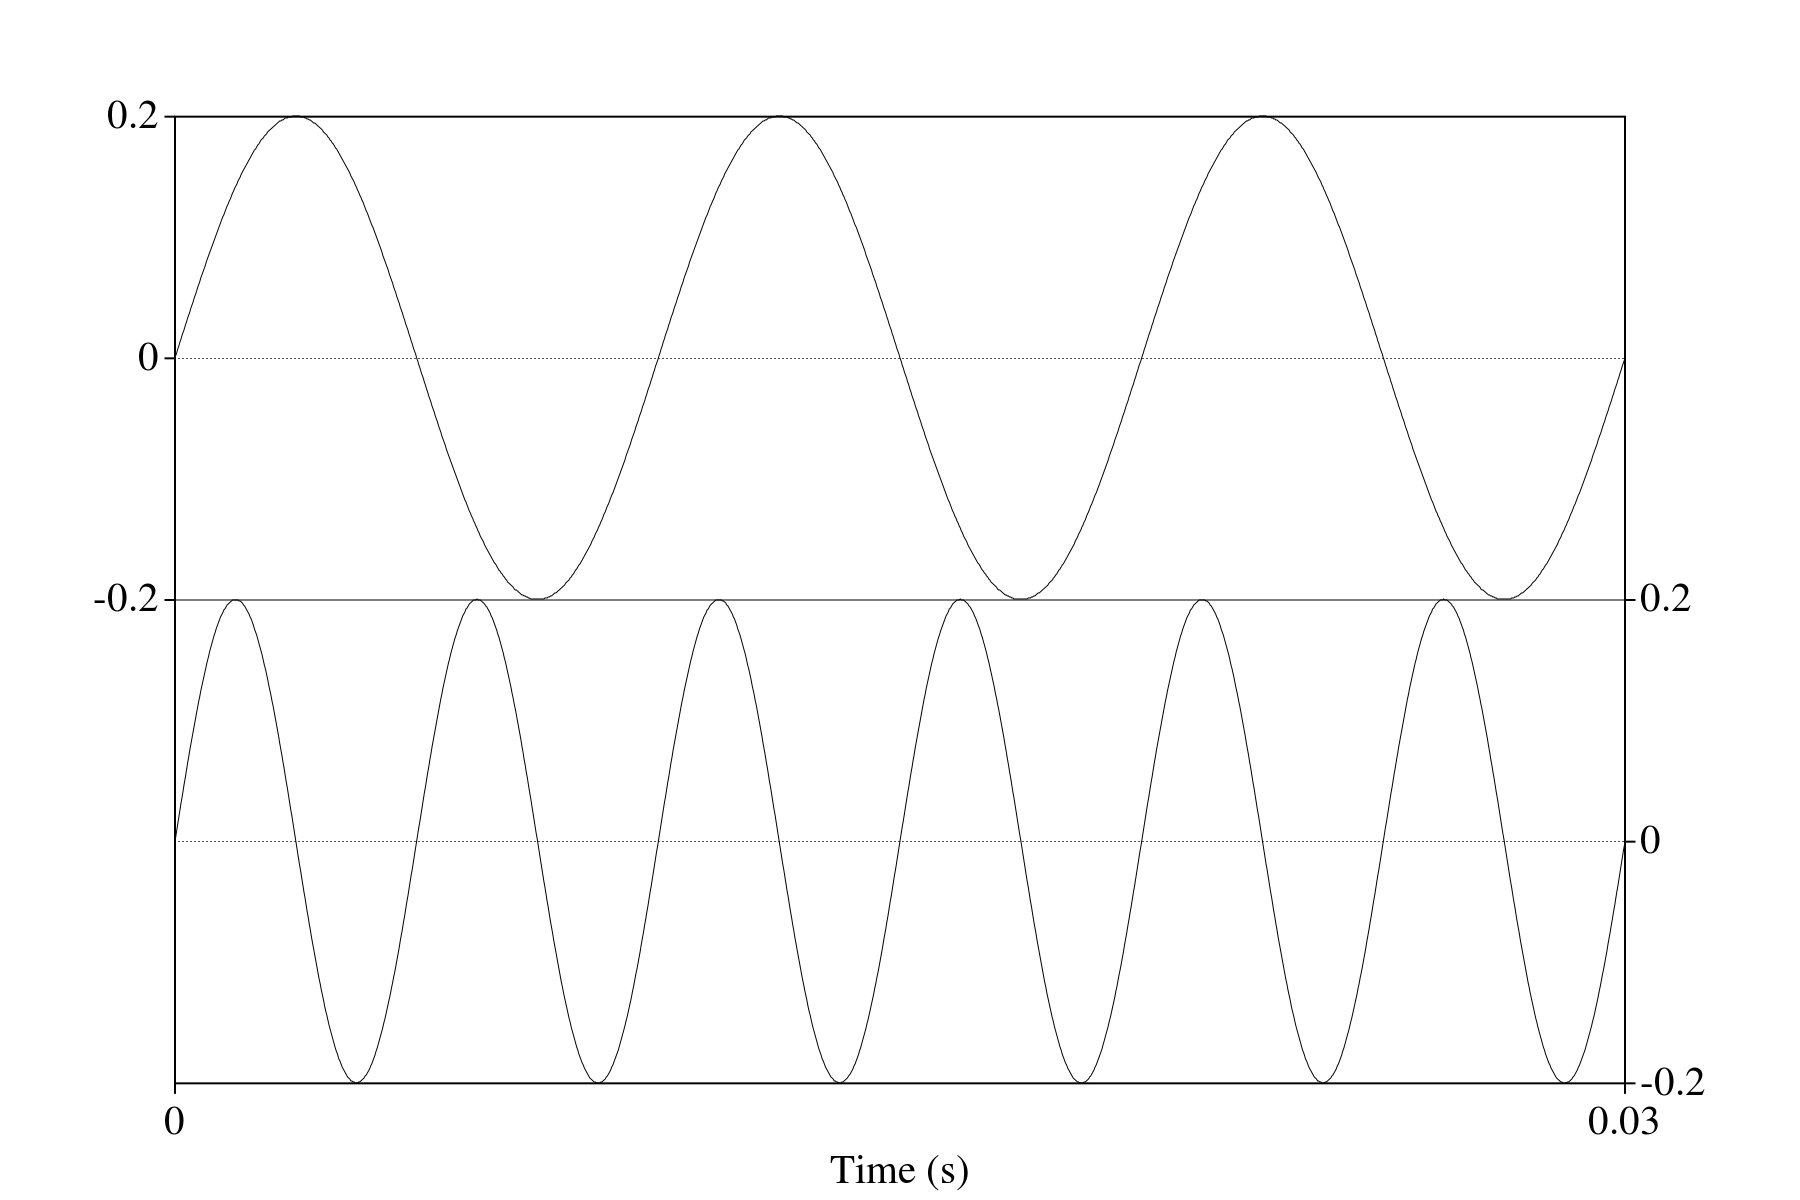
\includegraphics[width=\textwidth]{figure/basic-sound-frequency.png}
  \caption{Two waveforms showing a difference in frequency between the two signals.}
  \label{fig:basic-sound-frequency}
\end{subfigure}
%
\\[2ex]
\begin{center}
\begin{subfigure}{0.5\textwidth}
  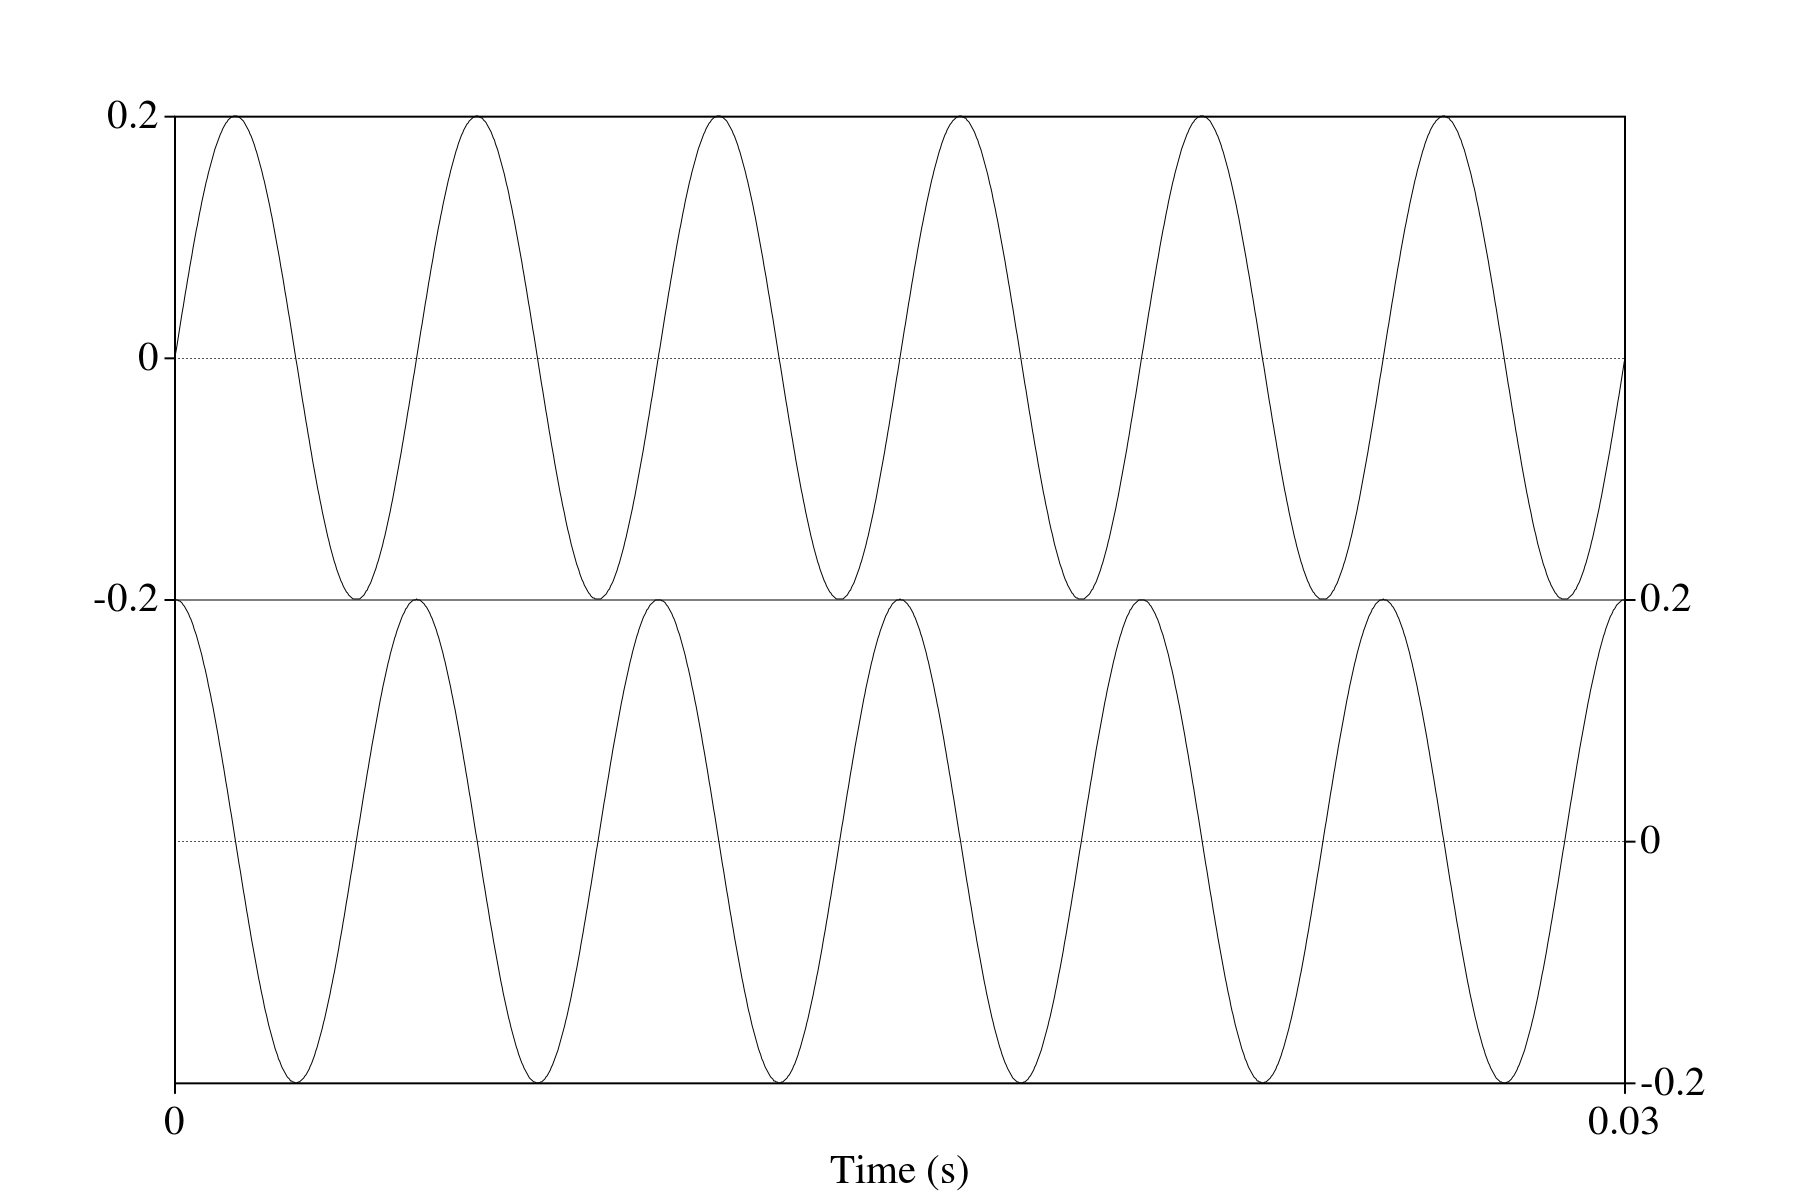
\includegraphics[width=\textwidth]{figure/basic-sound-phase.png}
  \caption{Two waveforms showing a difference in phase between the two signals.}
  \label{fig:basic-sound-phase}
\end{subfigure}
\end{center}
\caption{Waveforms demonstrating difference in amplitude, frequency, and phase.}
\label{fig:basic-sound-wave}
\end{figure}


\subsection{Overview of Anatomy and Physiology of the Peripheral Auditory System}

Prior to discussing the acoustic structure of speech, it is important to become familiar with the basic peripheral auditory system.  The peripheral auditory system is generally grouped into three primary categories, the outer ear, the middle ear, and the inner ear (cf. Figure \ref{fig:ear-anatomy}).  The outer ear includes the pinna, the ear canal, and the tympanic membrane (ie. the eardrum).  Air-transmitted sound vibrations, ie. pressure fluctuations, enter the ear canal through the opening at the pinna.  These then travel along the canal to vibrate the tympanic membrane, which passes the energy to the middle ear.  The middle ear includes the ossicles within the middle ear cavity.  The ossicles form a chain of three very small bones leading from the tympanic membrane to the cochlea. The external sound vibrations impose an oscillating force on the tympanic membrane, setting it into motion. This results in displacement at the ossicular chain, which then transforms the vibrations into a traveling wave passing along the basilar membrane within the fluid-filled cochlea of the inner ear (\cite{rosen:91}).

\begin{figure}[H]
\centering
  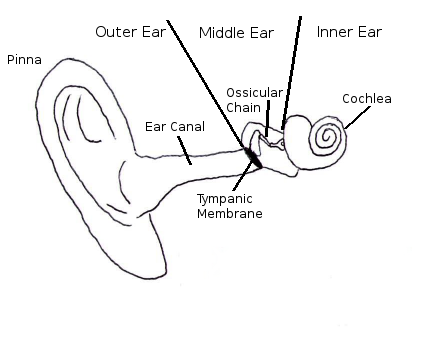
\includegraphics[width=.75\textwidth]{figure/ear-diagram.png}
  \caption{A diagram of the peripheral auditory system, including the outer ear, middle ear, and inner ear.}
  \label{fig:ear-anatomy}
\end{figure}

The inner ear is composed of the cochlea, and the semicircular canals and auditory and vestibular nerves (the latter three are not pictured).  The semicircular canals, and vestibular nerve don't play a part in audition (their primary function regards balance sensitivity).  The cochlea, a hard `shell' filled with fluid, receives the vibrations passed to it by way of the middle ear ossicles.%\footnote{The peripheral auditory system uses gas, solid, and liquid media to transmit acoustic vibrations.}  
The vibrations are passed into the fluid of the cochlea and travel along its length, transmitting hydro-mechanical energy to cells on the basilar membrane that are able to detect the displacement of the fluid by means of sensory membranes.  The basilar membrane serves as the base on which these sensory cells are fixed.  Depending on the location of the sensory cells along the basilar membrane, they respond to a different frequency of `sound', ie. fluid pressure fluctuation.  This placement of sensory cells `tuned' to detect a particular frequency band is called tonotopic organization.  This essentially allows the cochlea to perform a Fourier Transform - which extracts all the different frequency components from a wave - of the sound that is transmitted to it.  The auditory nerve carries electrical impulses from these sensory cells into the auditory cortex of the brain (\cite{rosen:91,celesia:15}). 

Of interest to this present study is the outer ear.  Typically, as described above, vibrations from the air will enter the ear canal through the opening at the pinna. Frequently, these vibrations take the form of human speech.

%However, vibrations from one's own speech are also transmitted via the bone, cartilage, and tissue of the head.  Regardless of source, sound vibrations entering into the ear canal will be altered by the shape of the ear canal, described more below.


\subsection{Acoustic Structure of Human Speech}

The structure of human speech draws from a collection of individual sounds (phonemes) that are strung together, encoding words, sentences, and more abstractly, meaning.  Each human language uses a subset of all possible phonemes.  Each phoneme is either considered `voiced' or `unvoiced'.  The acoustic properties of sounds in these two categories differ greatly (\cite{ladefoged:14}).


%
\begin{wrapfigure}{l}{0.5\textwidth}
\centering
  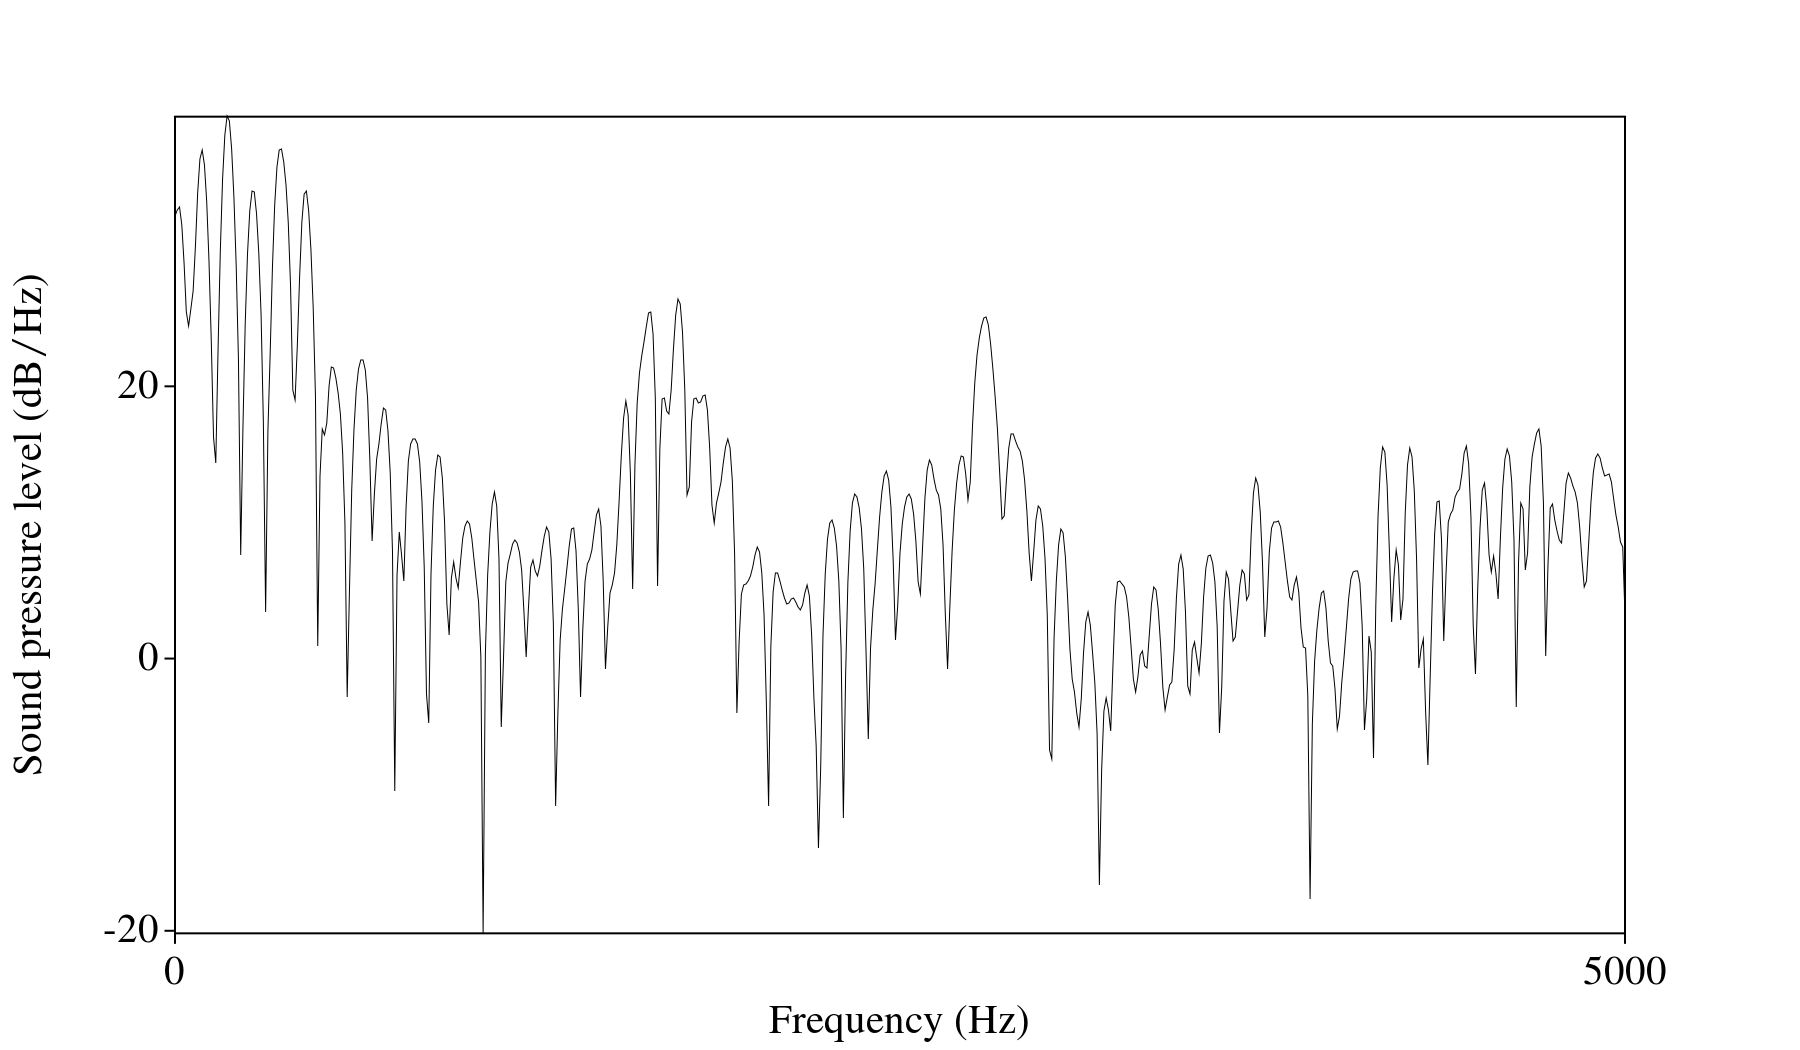
\includegraphics[width=0.5\textwidth]{figure/spctrm5k.png}
  \caption{Spectrum of the middle of an /I/ vowel.  Each `hump' is a separate narrow band of frequency, called a harmonic.}
  \label{fig:spctrm5k}
\end{wrapfigure}
%
Voiced speech is composed of narrow bands of acoustic energy, called harmonics, located along a frequency spectrum (cf. Fig \ref{fig:spctrm5k}).  In this sense, speech is considered a `complex' sound, because it is composed of energy at multiple frequencies.  Certain harmonics will be dampened by the vocal tract, leaving others relatively unfiltered.  A group of neighboring harmonics containing more energy than other harmonics are called formants.  The location, shape, and transition over time of these formants (among other more minor features) encodes speech information for voiced sounds.  This can be visualized in a spectrogram (cf. Fig. \ref{fig:spctgrm_citizen}).


\begin{figure}[H]
\begin{subfigure}{\textwidth}
  \centering
  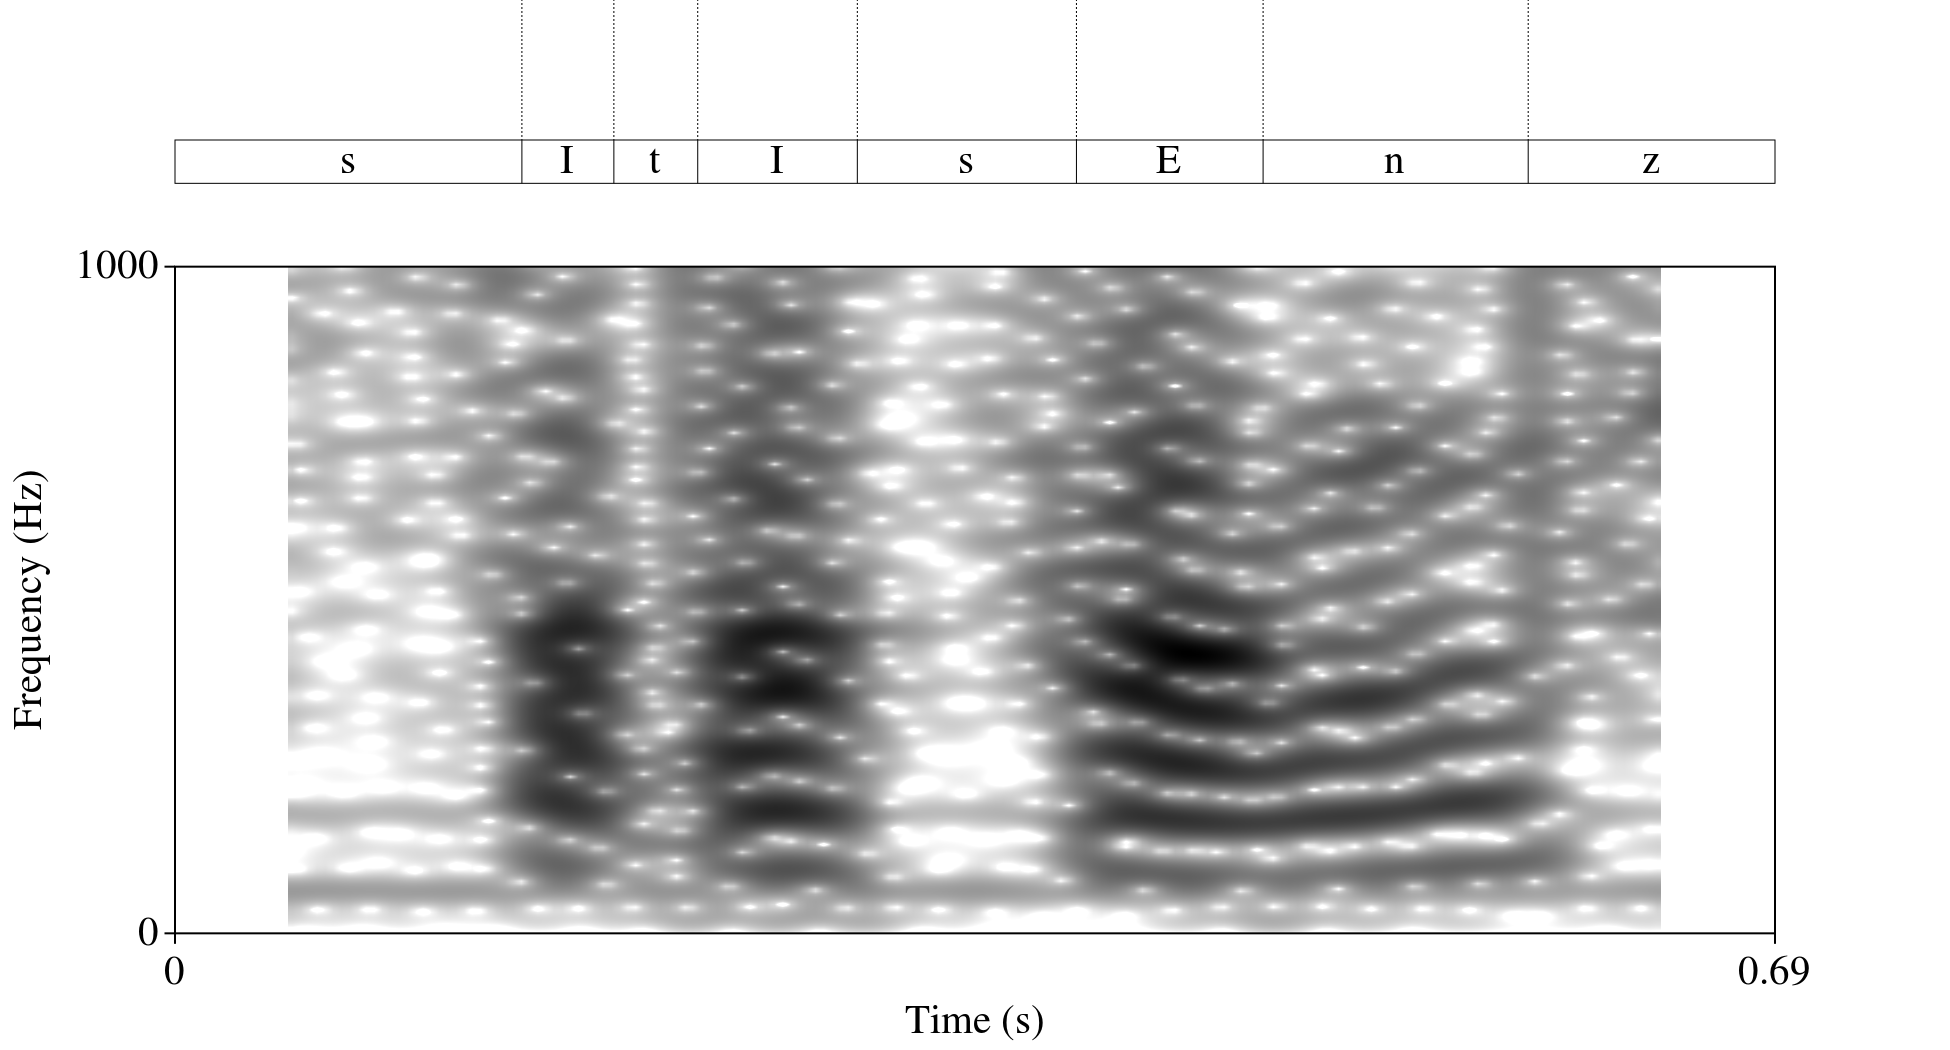
\includegraphics[width=0.85\textwidth]{figure/spctgrm1k.png}
  \caption{Zoomed to the 0-1kHz range for better visualization of harmonics.}
  \label{fig:spctgrm_citizen_1k}
\end{subfigure}%
\hfill
\begin{subfigure}{0.95\textwidth}
  \centering
  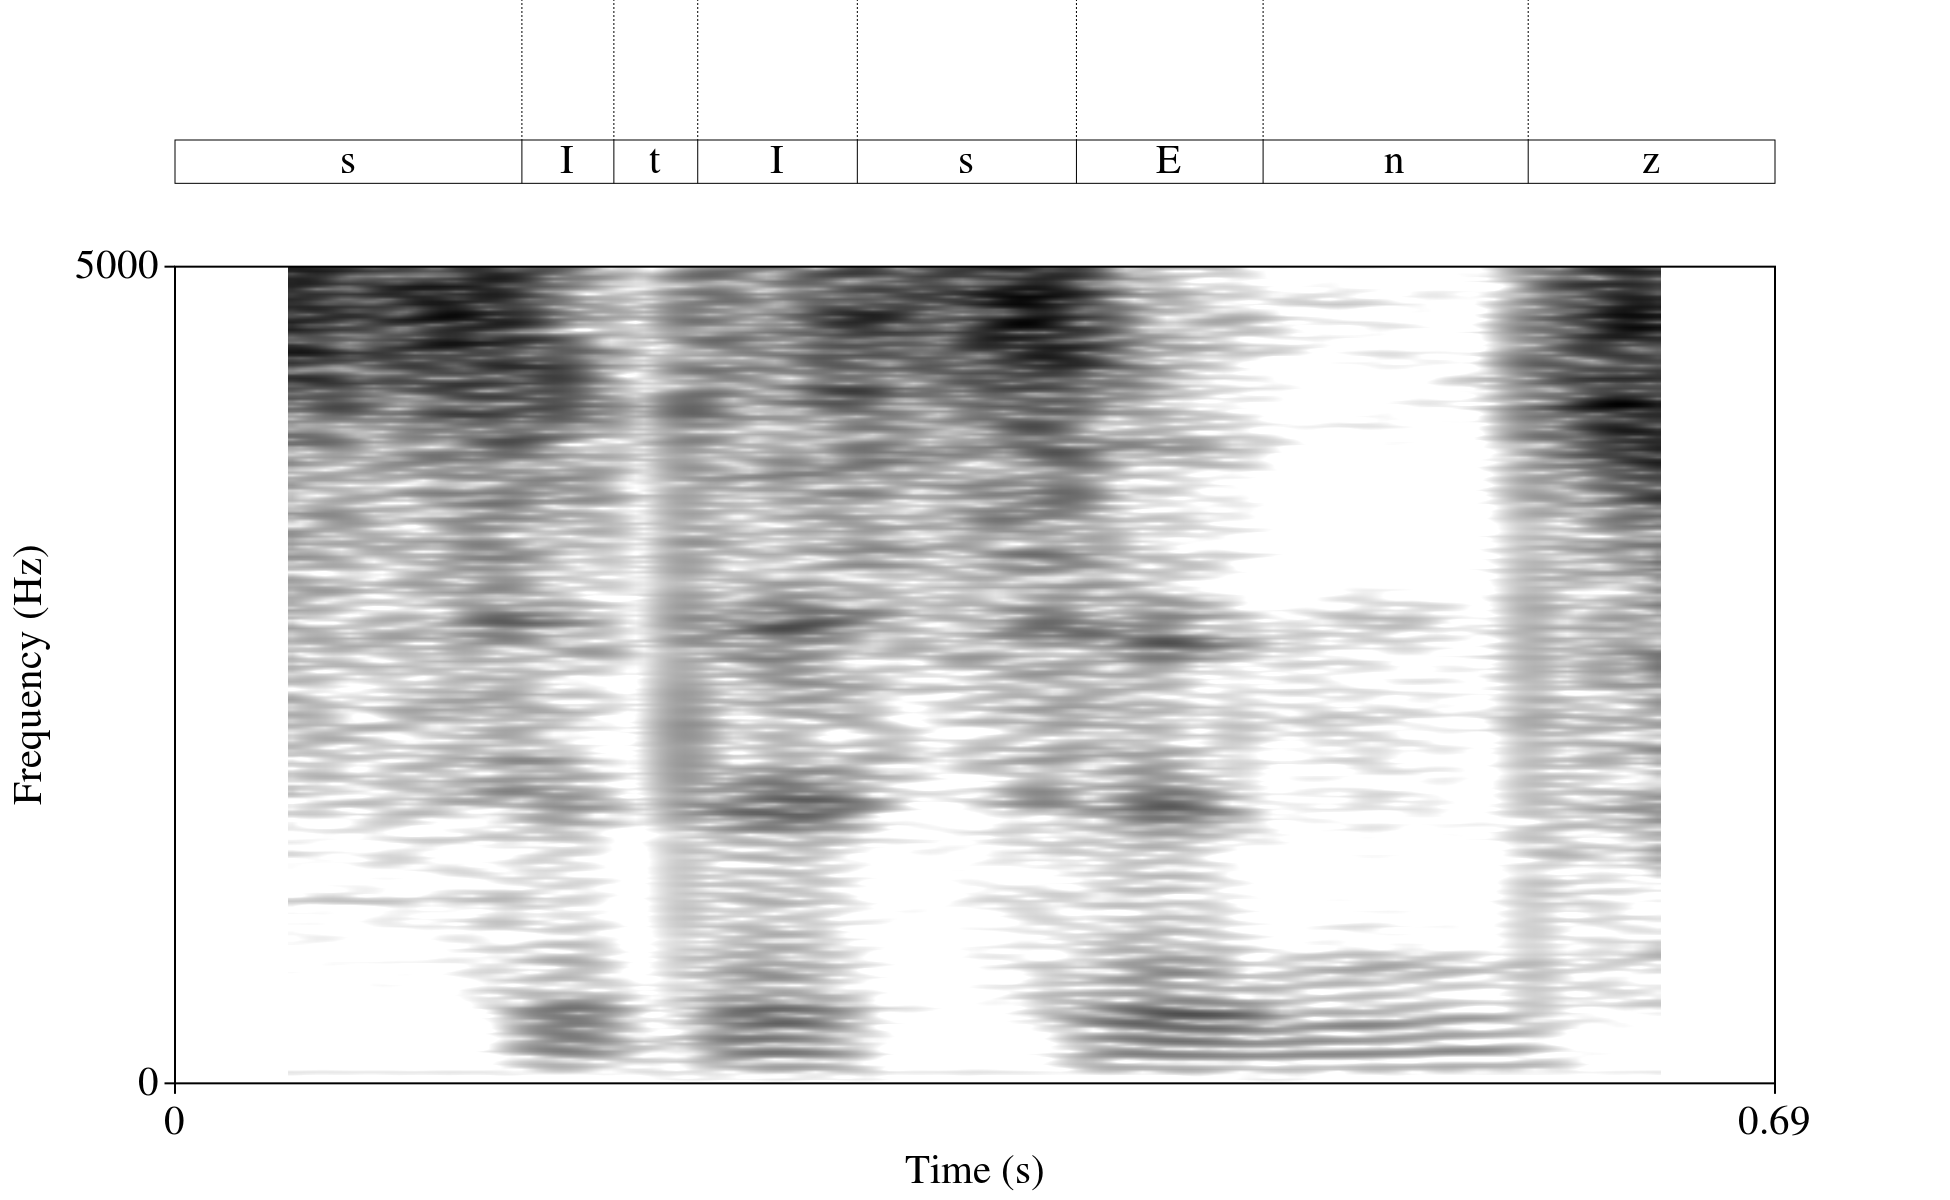
\includegraphics[width=0.85\textwidth]{figure/spctgrm5k.png}
  \caption{Zoomed to a more standard 0-5kHz range.}
  \label{fig:spctgrm_citizen_5k}
\end{subfigure}
\caption{Narrow-band spectrogram of the word `citizens' with phonetic transcription above.  Frequency is on the y-axis, time is on the x-axis, and amplitude is shown in grayscale on the graph; the darker an area of the graph, the greater the amplitude. Phoneme boundaries are approximate.}
\label{fig:spctgrm_citizen}
\end{figure}

For unvoiced speech, the information used to recognize and categorize the speech sound is likely found in the turbulent frication generally centered in higher frequencies (cf. Fig. \ref{fig:spctgrm_s}), although some of the information can be found in lower frequencies or found in surrounding voiced information, such as formant transitions into and out of the sound (\cite{halle:57,lindblom:63,stevens:78,willi:17}).  Generally, most speech information used by the human auditory system can be found in frequencies below 5.0-8.0 kHz.

\begin{wrapfigure}{l}{0.5\textwidth}
\centering
  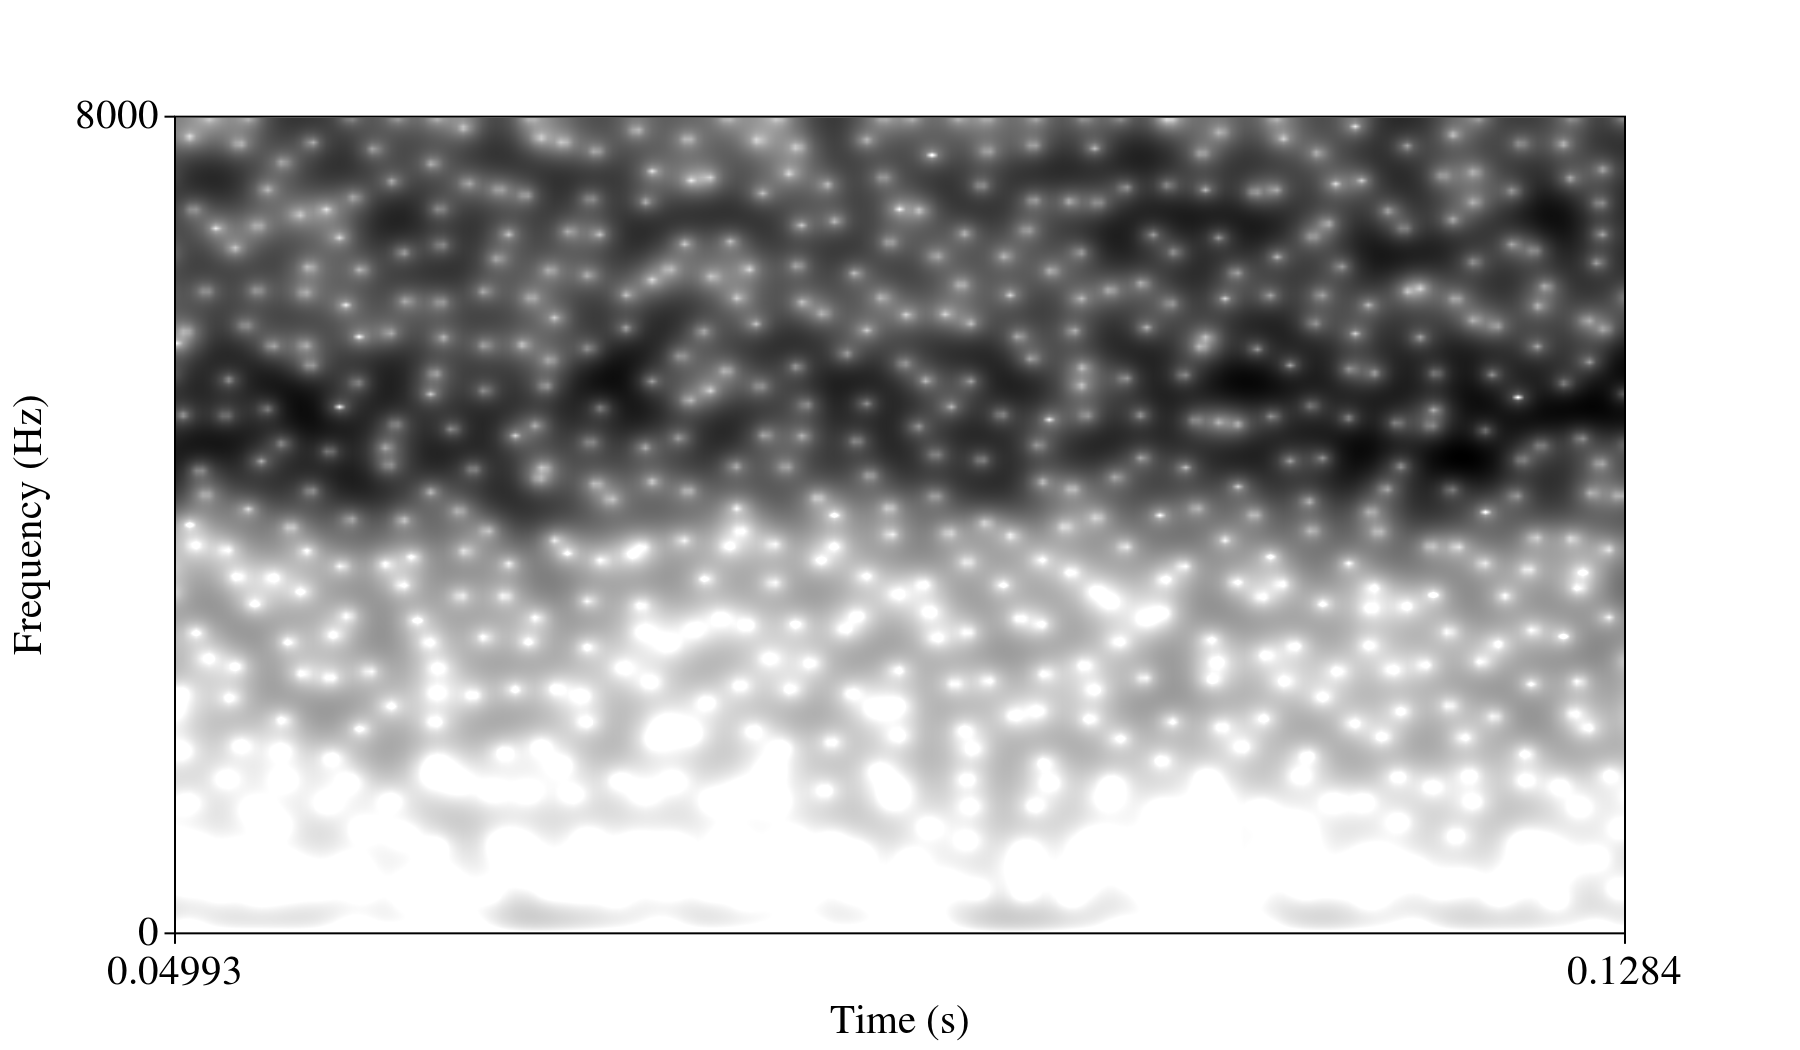
\includegraphics[width=0.5\textwidth]{figure/spctgrm_s.png}
  \caption{Spectrum of the initial /s/ in `citizens'. Zoomed to range of 0-8 kHz for visualization of high frequency energy.}
  \label{fig:spctgrm_s}
\end{wrapfigure}
%
The human auditory cortex has the remarkable ability to (a) transduce these sounds, which often only last from tens to a few hundreds of milliseconds in duration, (b) partition the stream of sounds into their respective words, and (c) string the words together into a sentence and pull meaning from it - all in real time (\cite{celesia:15}).  Nevertheless there are occasionally recognition errors, which can occur anywhere along this auditory chain.  %The `lowest' level in this chain in which errors occur is the recognition and identification of sounds in the auditory cortex.  
There are a host of reasons why these errors might occur, yet the studies presented throughout this dissertation focus on additive noise interfering with the speech signal or signal distortion via passage of speech through a speaker's head.

\subsection{Acoustics of Complex Signals}

Humans use the amplitude and frequency of pressure fluctuations to perceive sound (\cite{rosen:91}). When sound travels through a medium from Source \textit{A}, there is nothing that prevents these pressure fluctuations of Source \textit{A} from acoustically mixing with the pressure fluctuations originating from Source \textit{B}.  For example, in Figure \ref{fig:sound-wave-addition}, Source \textit{A} produces a simple wave with a frequency of 100 Hz.  Source \textit{B} produces a simple wave with a frequency of 200 Hz.  If the waves from the two sources reach each other and overlap, a single wave is produced which would look similar to the one in Figure \ref{fig:sound-wave-addition-combined}.  This sound wave now has two components - a tone at 100 Hz and a tone at 200 Hz.

\begin{figure}[H]
\begin{subfigure}{0.5\textwidth}
  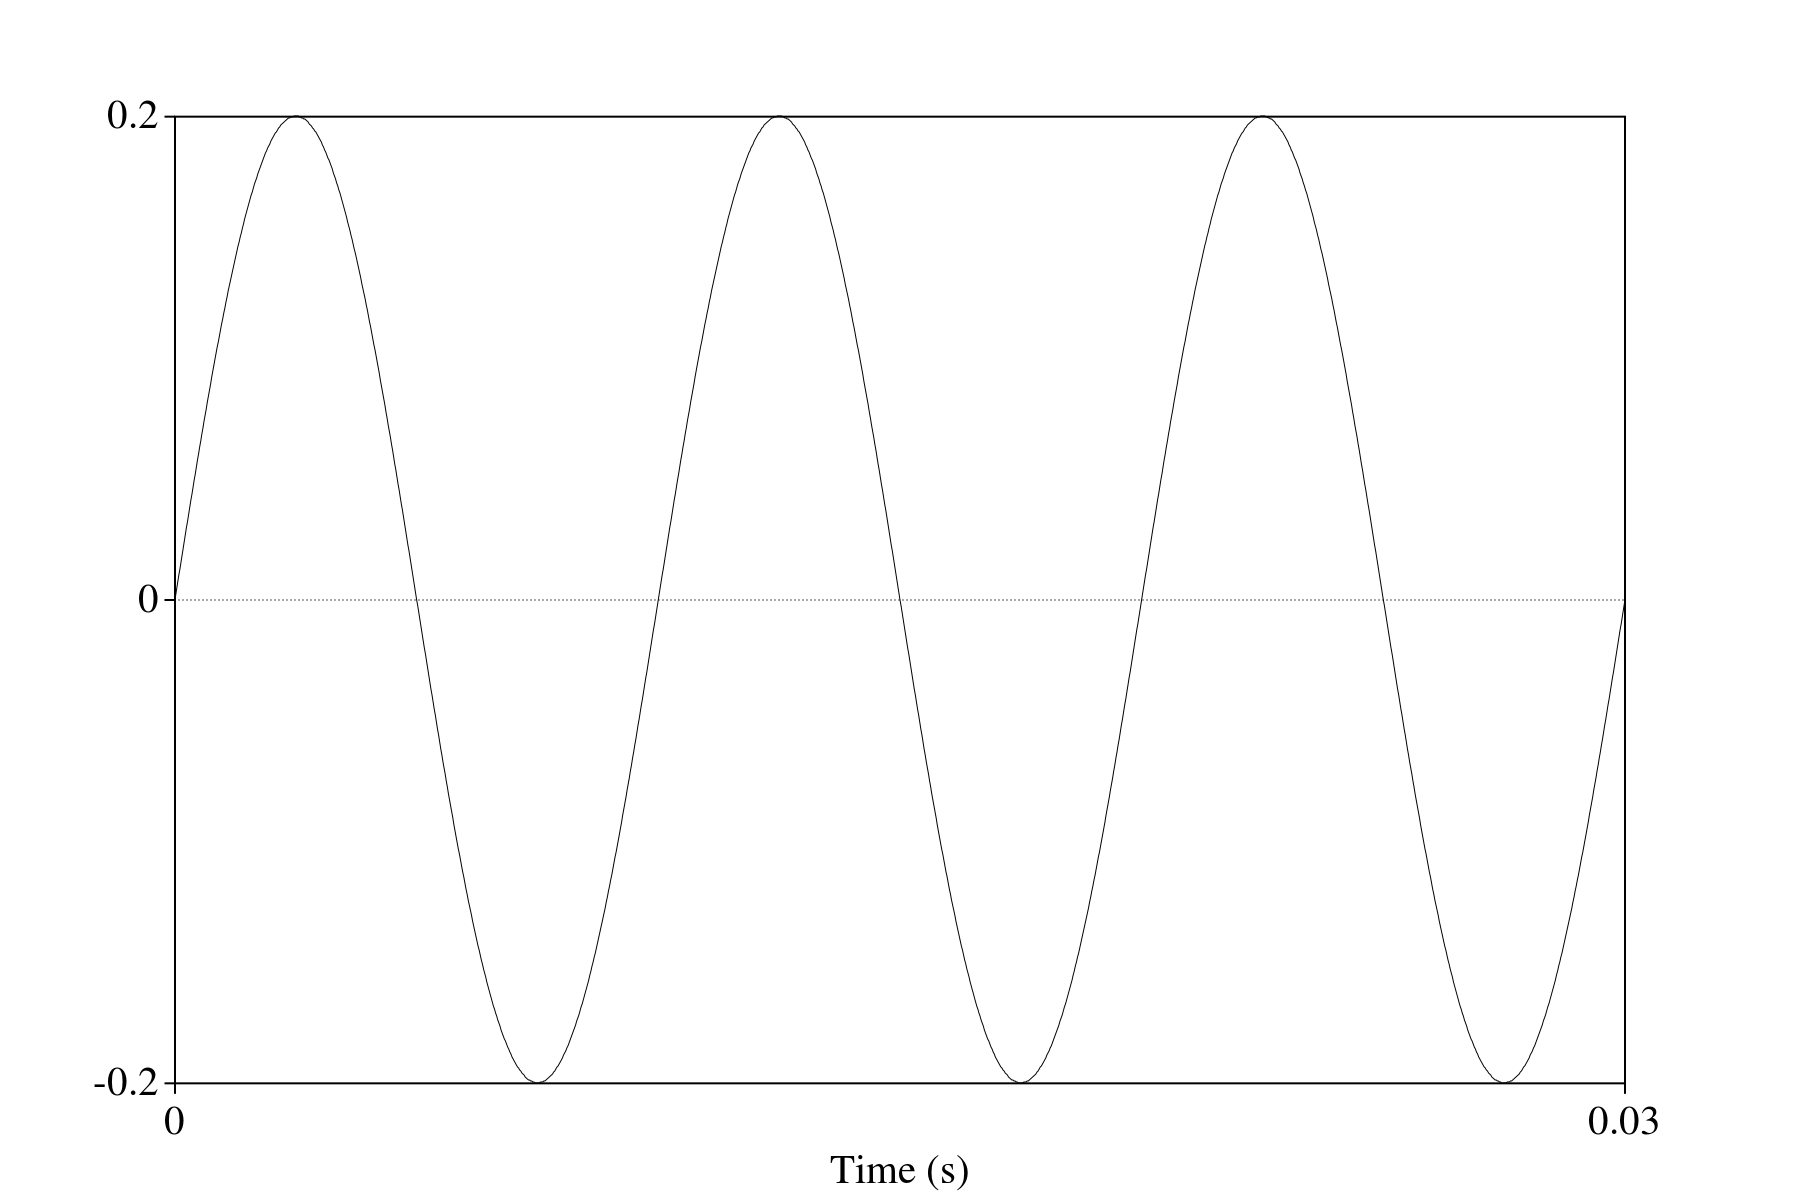
\includegraphics[width=\textwidth]{figure/basic-sound-wave.png}
  \caption{A basic sound wave from source \textit{A} at a frequency of 100 Hz.}
  \label{fig:sound-wave-A}
\end{subfigure}
\qquad
\begin{subfigure}{0.5\textwidth}
  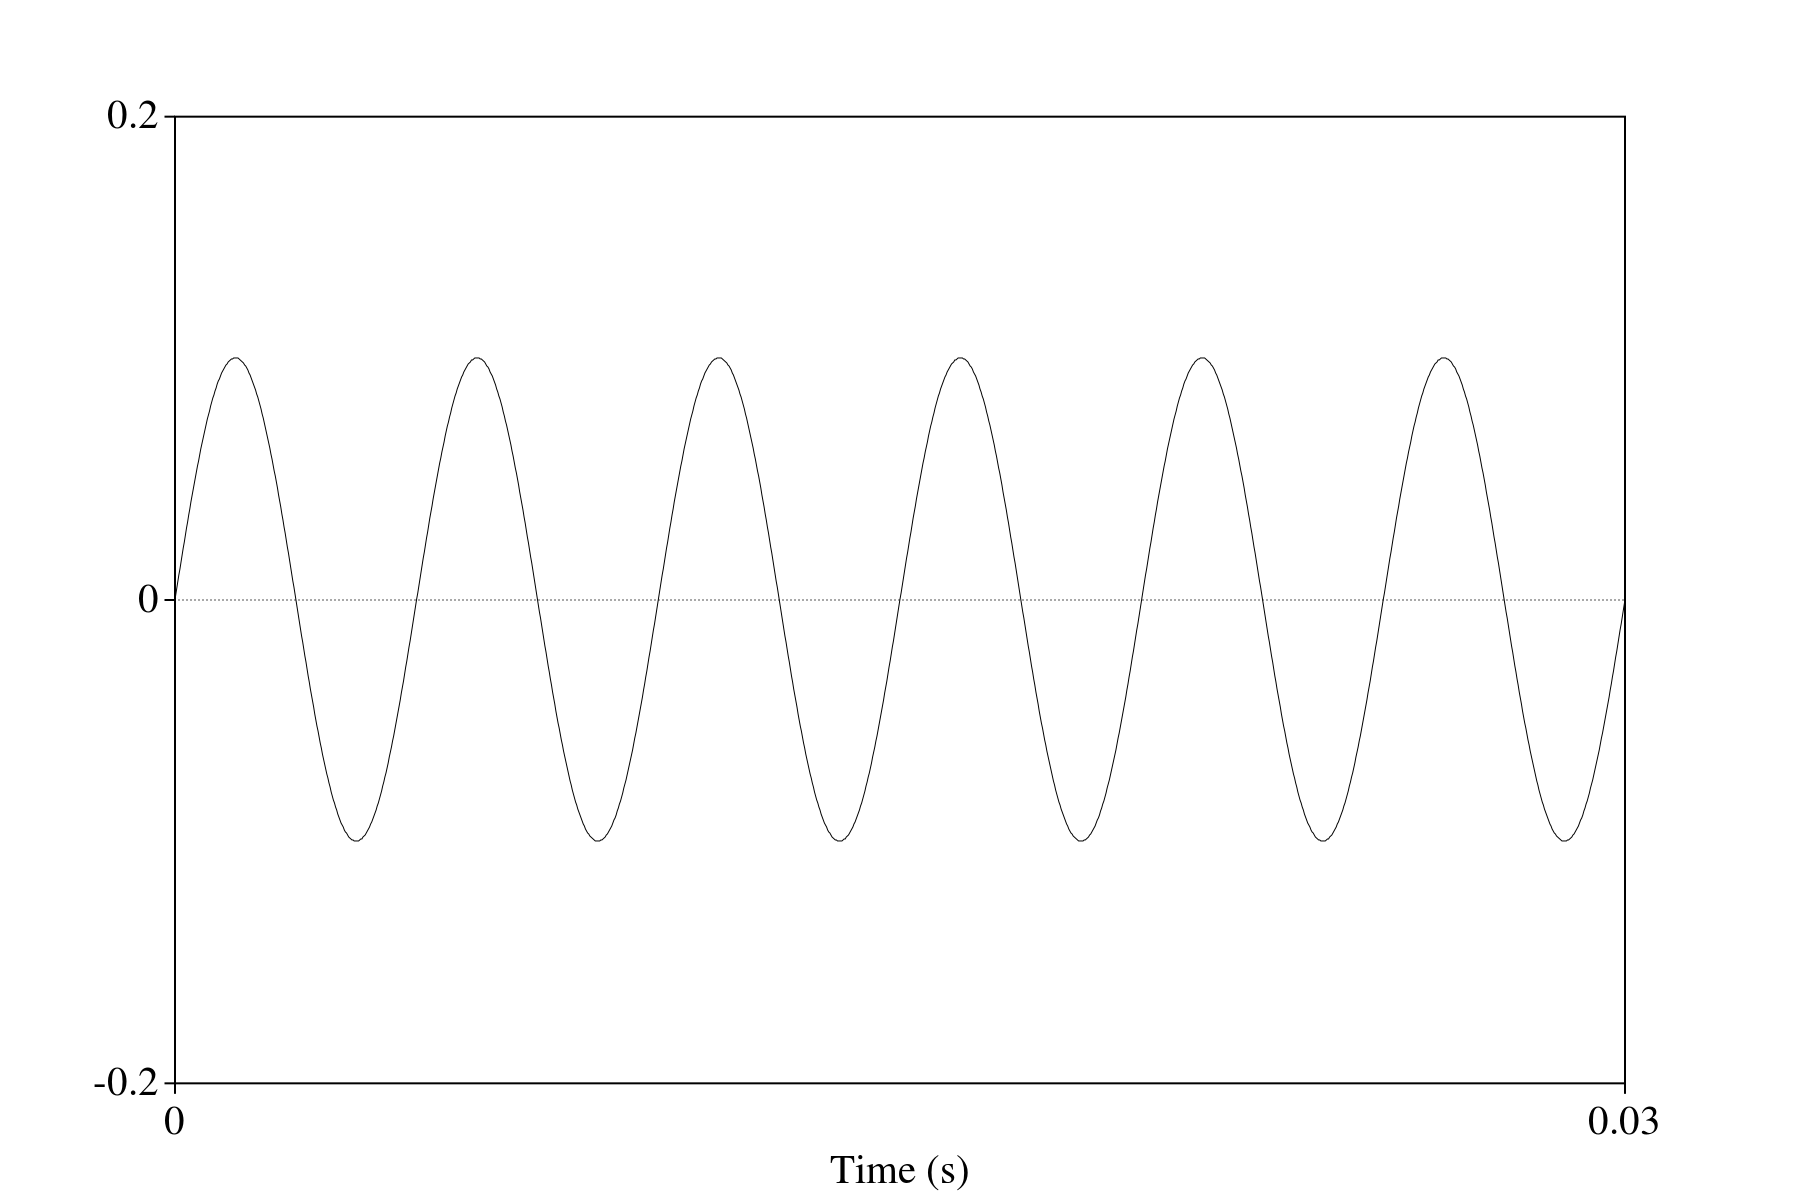
\includegraphics[width=\textwidth]{figure/sound-wave-addition-200hz.png}
  \caption{A basic sound wave from source \textit{B} at a frequency of 200 Hz, with half the amplitude of the simple sound wave from source \textit{A}.}
  \label{fig:sound-wave-B}
\end{subfigure}
%
\\[2ex]
\begin{center}
\begin{subfigure}{0.5\textwidth}
  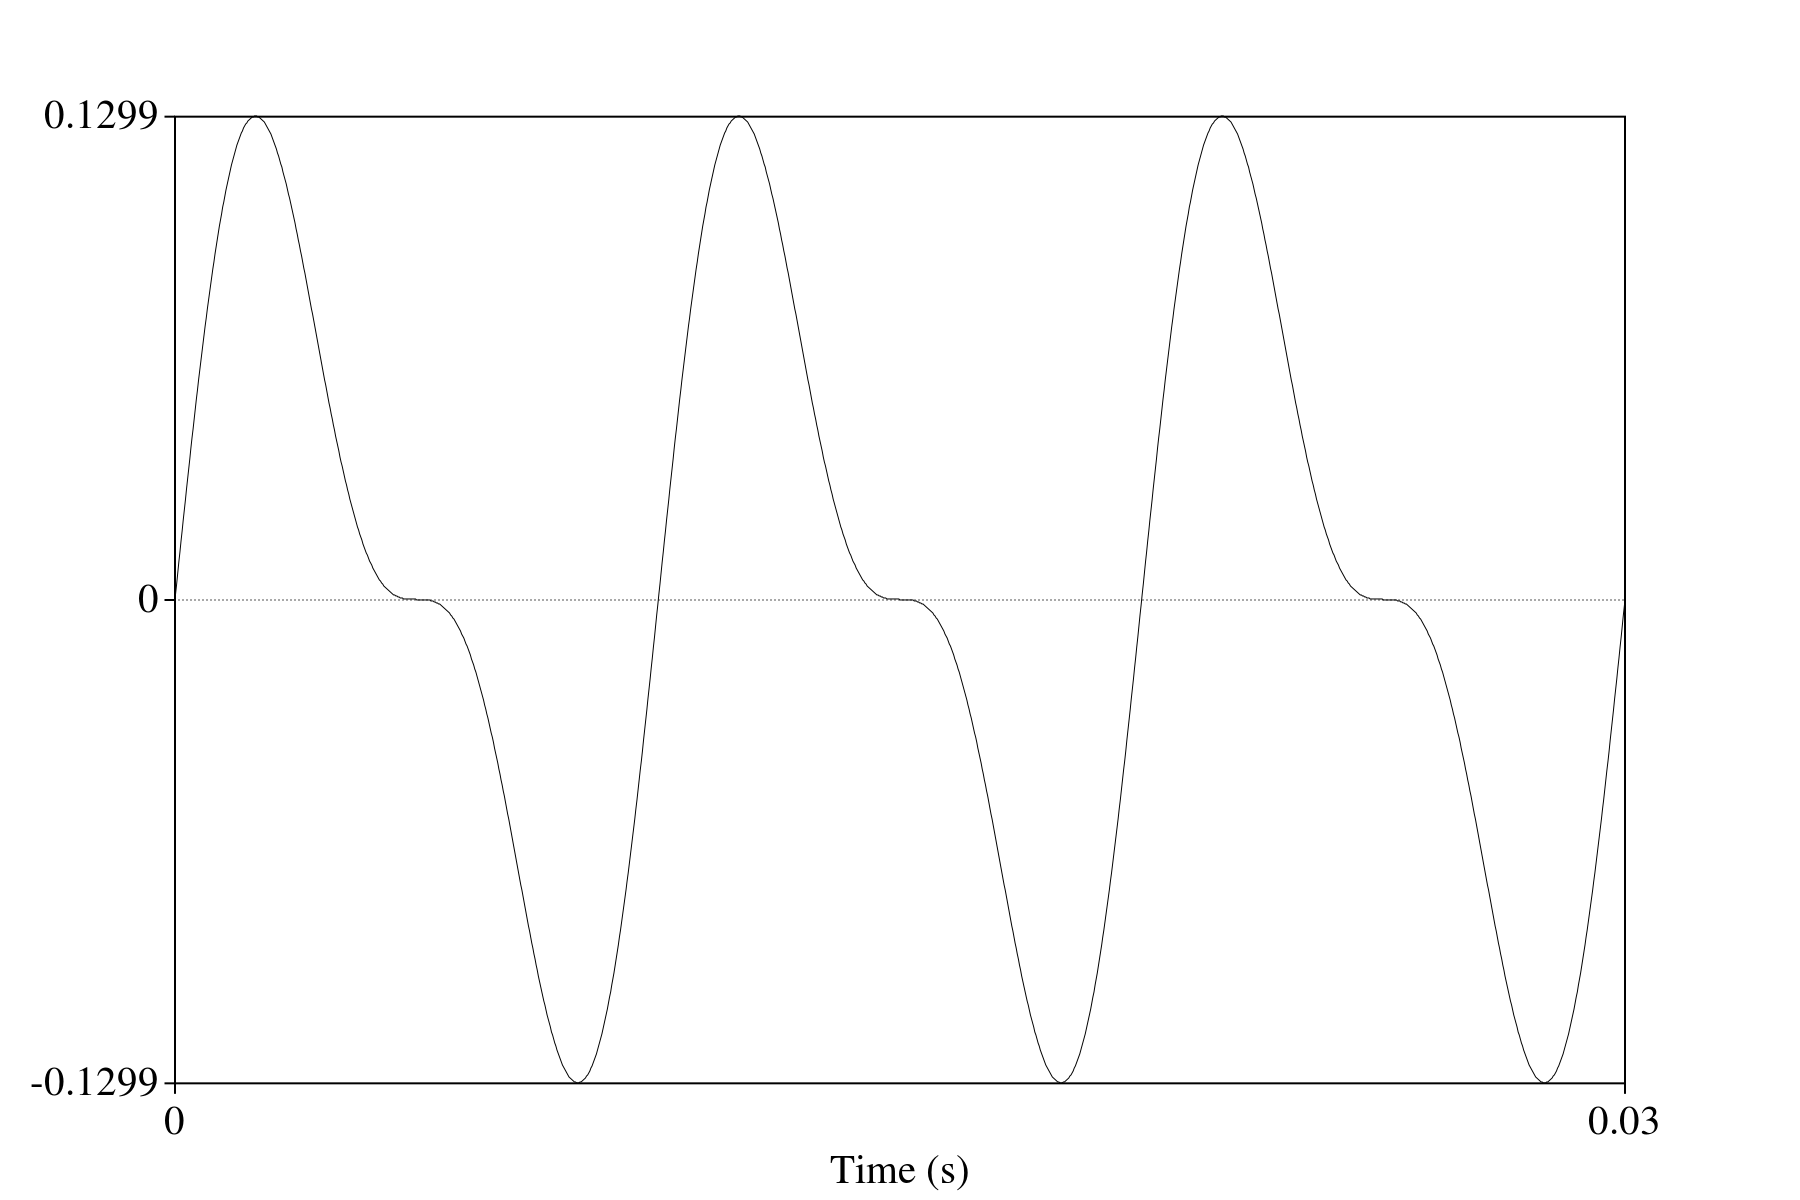
\includegraphics[width=\textwidth]{figure/sound-wave-addition-combined.png}
  \caption{The resulting complex wave from the combination of the wave from source \textit{A} and source \textit{B}.}
  \label{fig:sound-wave-addition-combined}
\end{subfigure}
\end{center}
\caption{Demonstration of the combination of two waves of different frequency and amplitude.}
\label{fig:sound-wave-addition}
\end{figure}

As previously mentioned, phase does not play a significant role in human audition, yet is a factor in the formation of a wave from the addition of multiple sound sources.  If Source \textit{B} (cf. Figure \ref{fig:wave-out-of-phase}) produces, instead, a wave of the same frequency and amplitude as the wave from Source \textit{A}, but they are completely `out of phase', ie. the pressure value of the waves at any given time is in direct opposition.  If these waves were combined, it would result in a complete elimination of sound (cf. Fig. \ref{fig:wave-out-of-phase-added}).

\begin{figure}[H]
\begin{subfigure}{0.5\textwidth}
  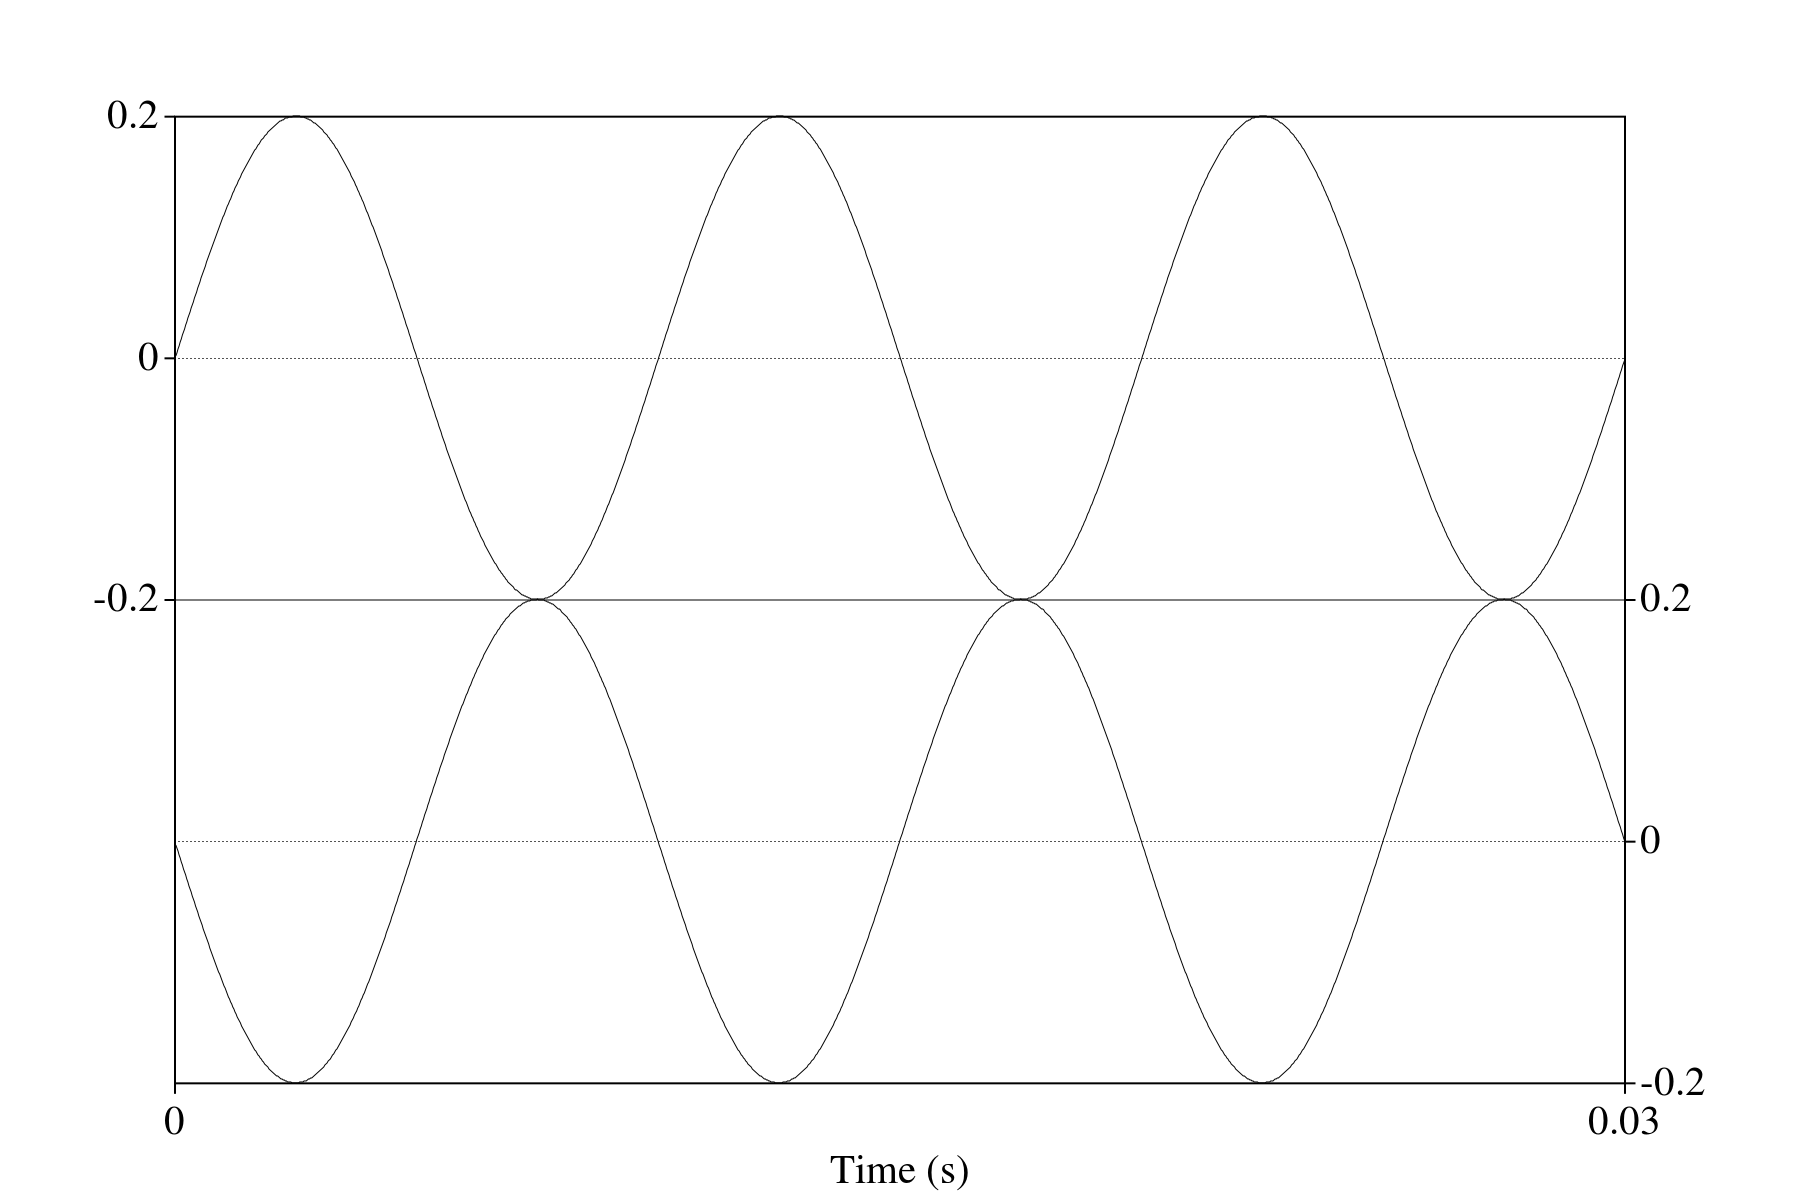
\includegraphics[width=\textwidth]{figure/wave-out-of-phase.png}
  \caption{Two sound waves with frequency of 100 Hz and the same amplitude, completely out of phase.}
  \label{fig:wave-out-of-phase}
\end{subfigure}
\qquad
\begin{subfigure}{0.5\textwidth}
  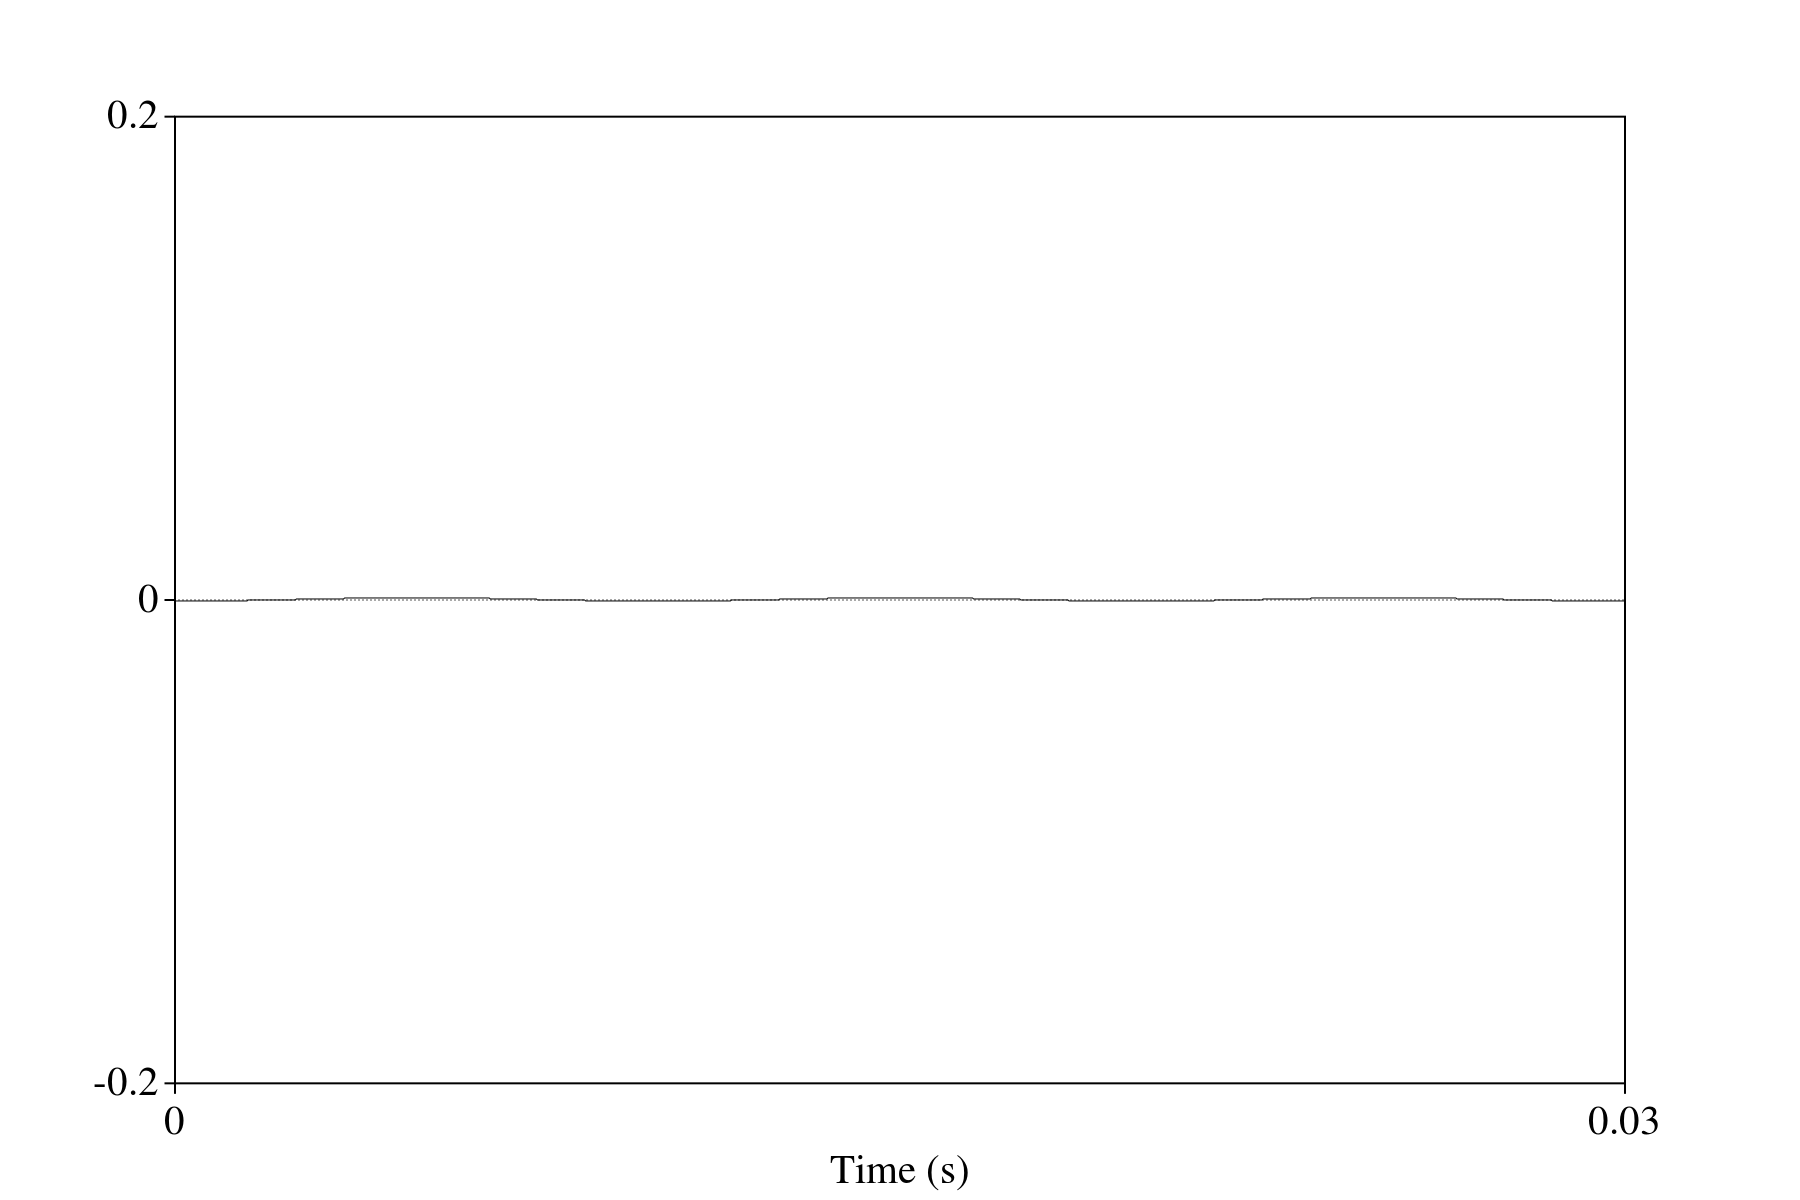
\includegraphics[width=\textwidth]{figure/wave-out-of-phase-added.png}
  \caption{The sound wave resulting from the combination of the two out of phase waves in Fig. \ref{fig:wave-out-of-phase}.}
  \label{fig:wave-out-of-phase-added}
\end{subfigure}
\caption{Demonstration of the combination of two completely out-of-phase waves with the same amplitude and frequency.}
\end{figure}

It is not very often that two waves of the exact same frequency and amplitude, with exactly opposing phase, meet in such a way to completely negate.  However, varying degrees of negation and alteration occur constantly due to phase and interacting sound waves.  For example, if the 100 Hz wave from Figure \ref{fig:sound-wave-addition} were combined with a 200Hz wave with a slightly shifted phase, a different wave would be produced, seen in Figure \ref{fig:sound-combined-shifted-phase}.  

The combination of waves from multiple sound sources increases greatly in complexity as the number of sources increases, and the as sounds originating from a single source is itself complex (ie. containing multiple frequency elements), such as speech.  Speech rarely occurs in isolation from from all external, interacting sound, yet we are still able to largely understand speech in everyday environments; for example, it is generally easy for humans to understand the speech of an interlocutor while sitting on a bench at a park.

The auditory system is well tuned to identify separate sources, even complex ones, like speech. Despite the shifted phase in Figure \ref{fig:sound-shifted-phase}, the human auditory system would still be able to detect and identify two separate waves.  While it undoubtedly plays a part, the differences in phase of combined signals does not normally completely negate a signal, nor render it unintelligible.  It is for this reason, and the complexity of phase calculations, that most efforts to remove noise from speech ignore the phase component.

\begin{figure}[H]
\begin{subfigure}{0.5\textwidth}
  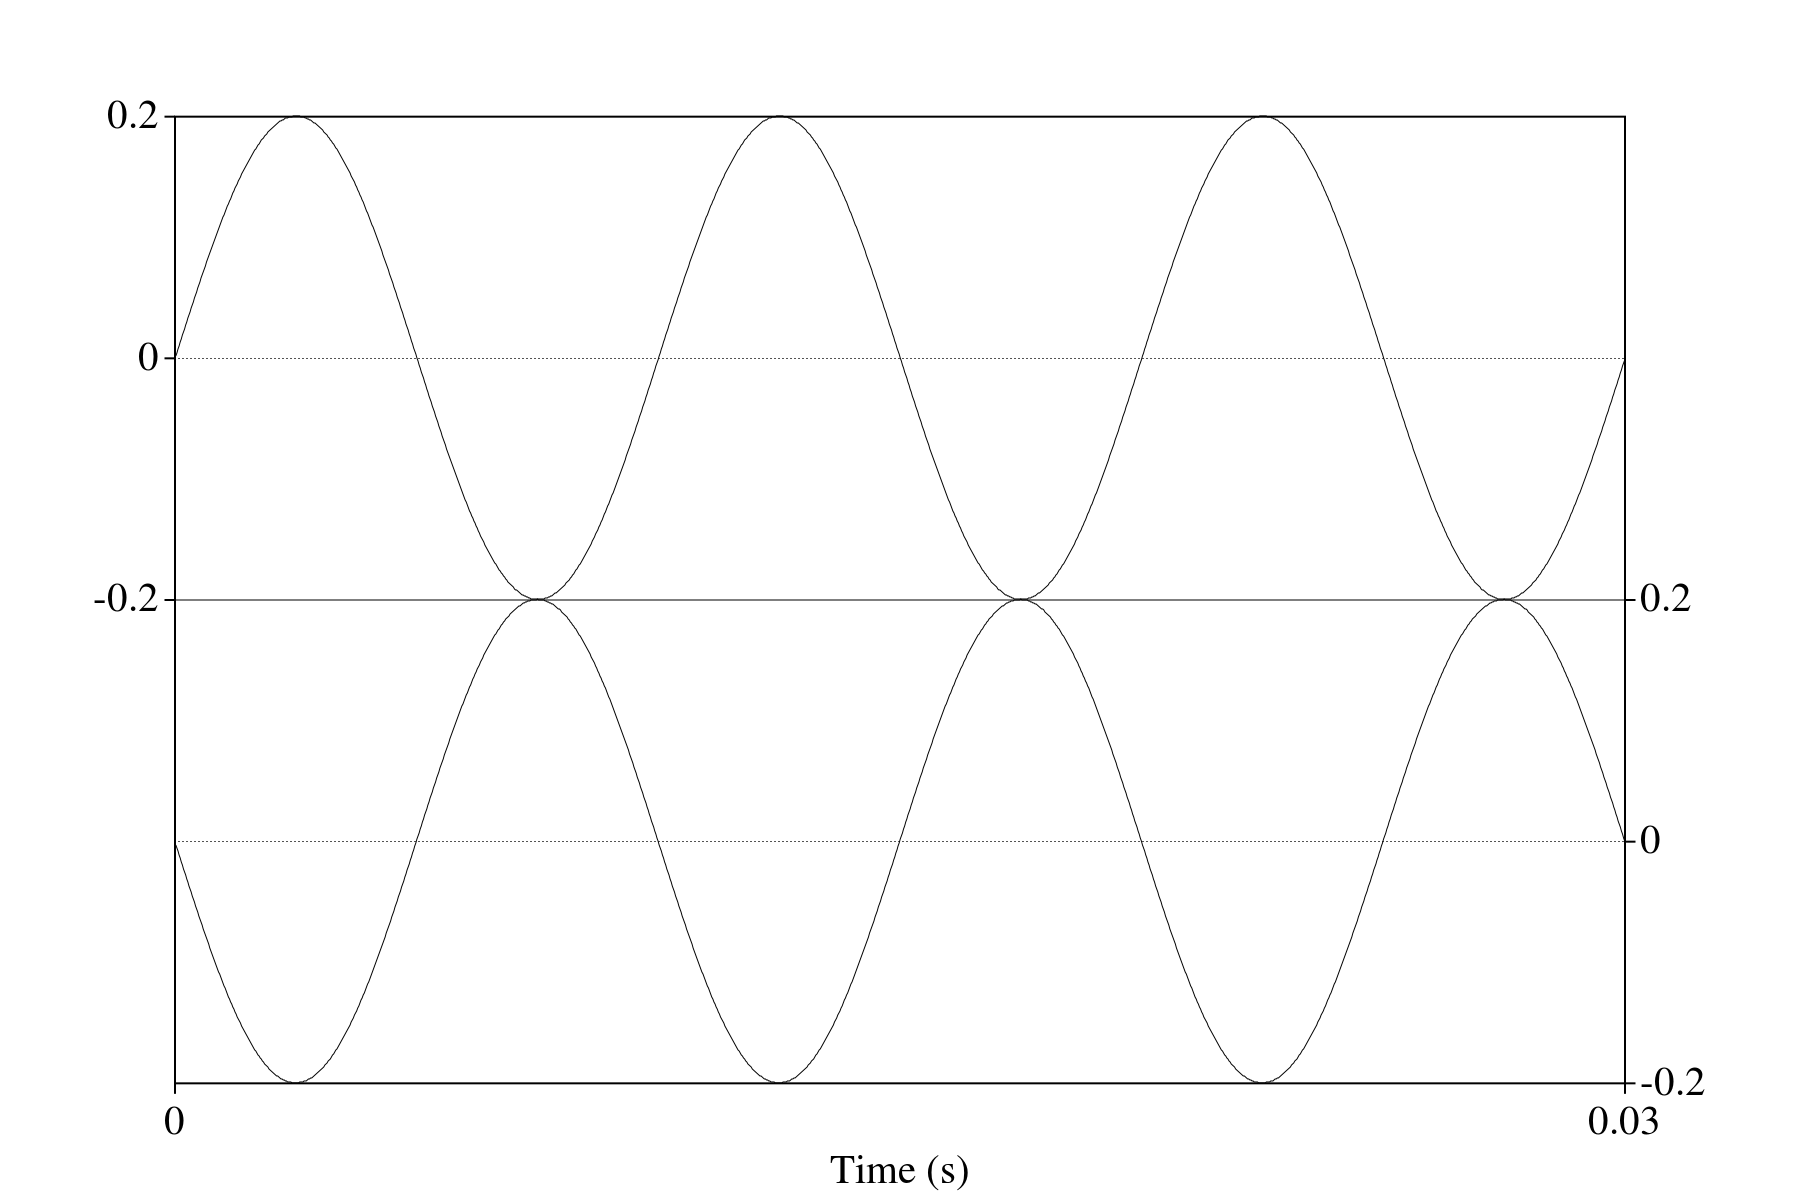
\includegraphics[width=\textwidth]{figure/wave-out-of-phase.png}
  \caption{Two sound waves with frequency of 100 Hz and the same amplitude, completely out of phase.}
  \label{fig:wave-out-of-phase2}
\end{subfigure}
\qquad
\begin{subfigure}{0.5\textwidth}
  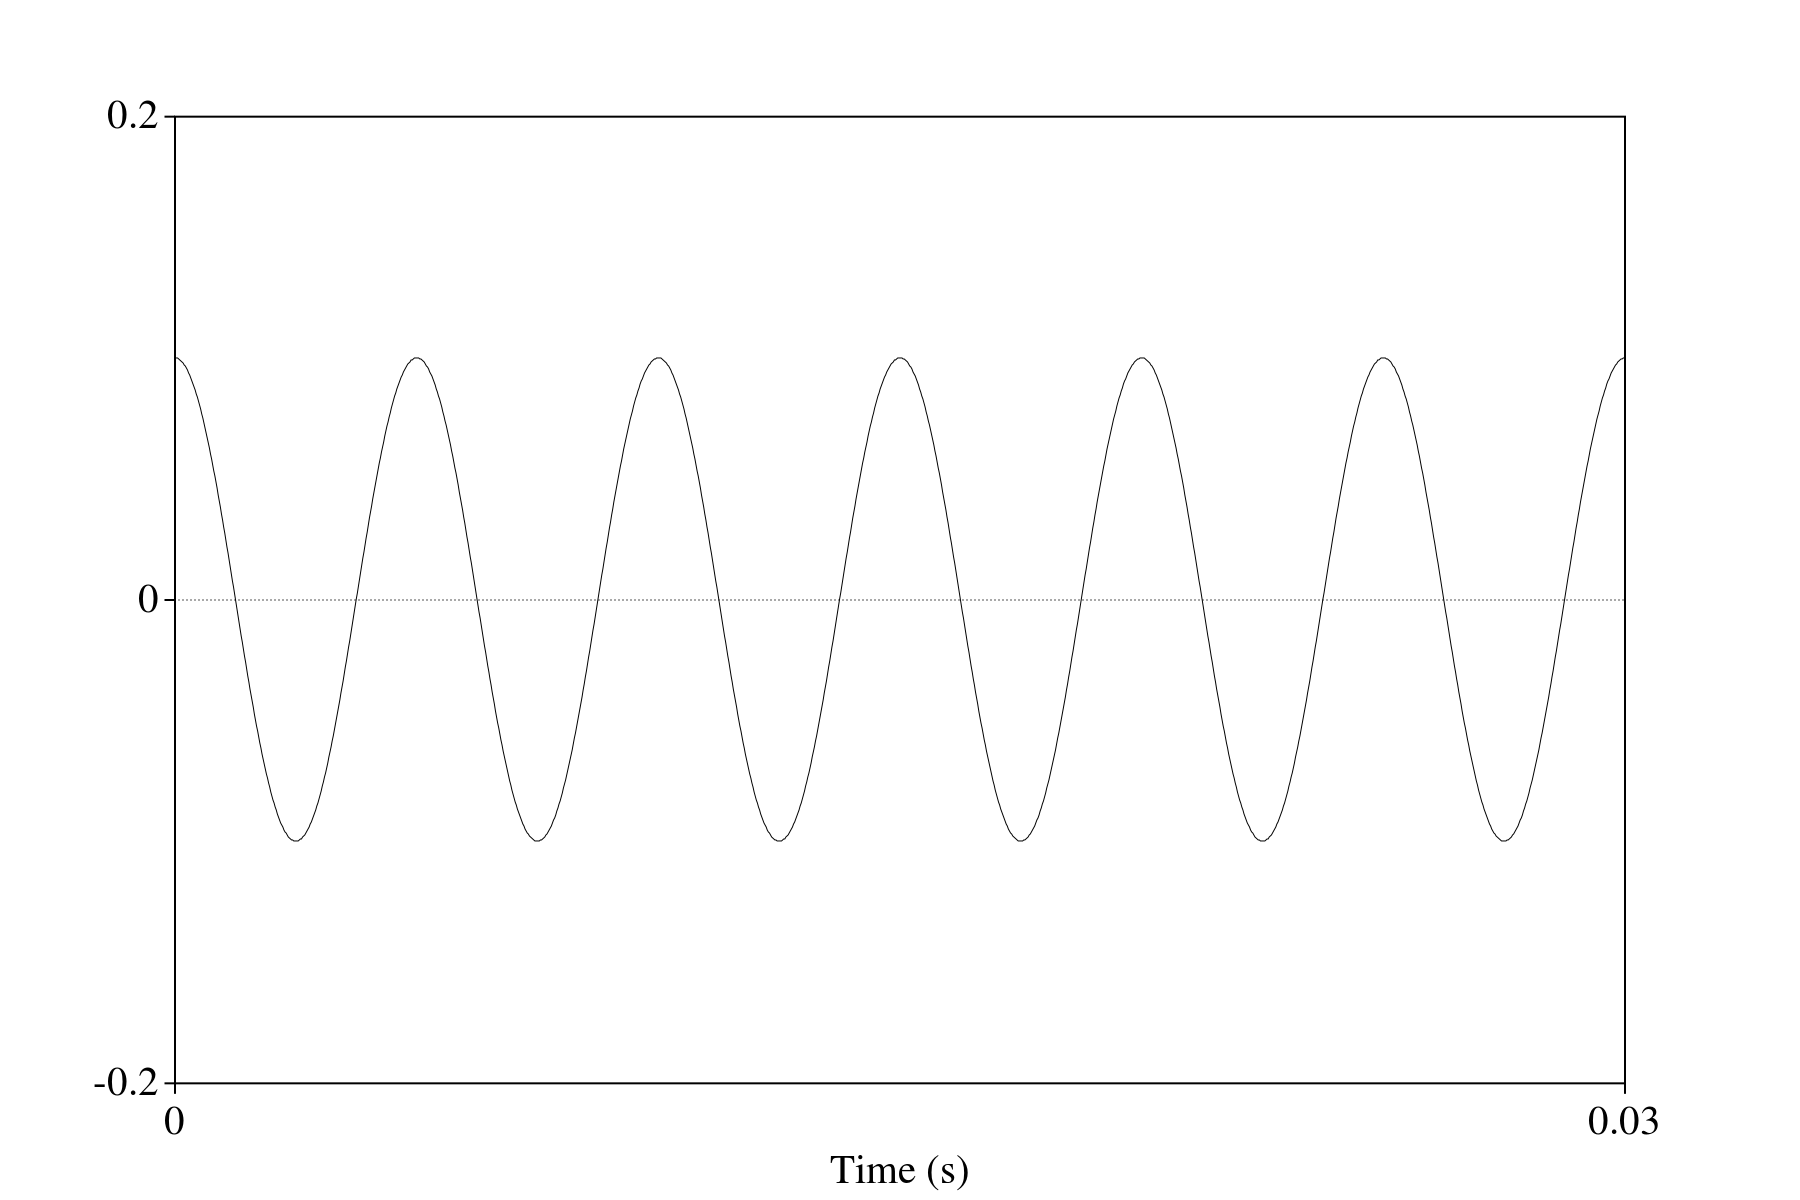
\includegraphics[width=\textwidth]{figure/sound-wave-addition-200hz-shifted.png}
  \caption{The sound wave resulting from the combination of the two out of phase waves in Fig. \ref{fig:wave-out-of-phase}.}
  \label{fig:wave-addition-200hz-shifted}
\end{subfigure}
%
\begin{center}
\begin{subfigure}{0.5\textwidth}
  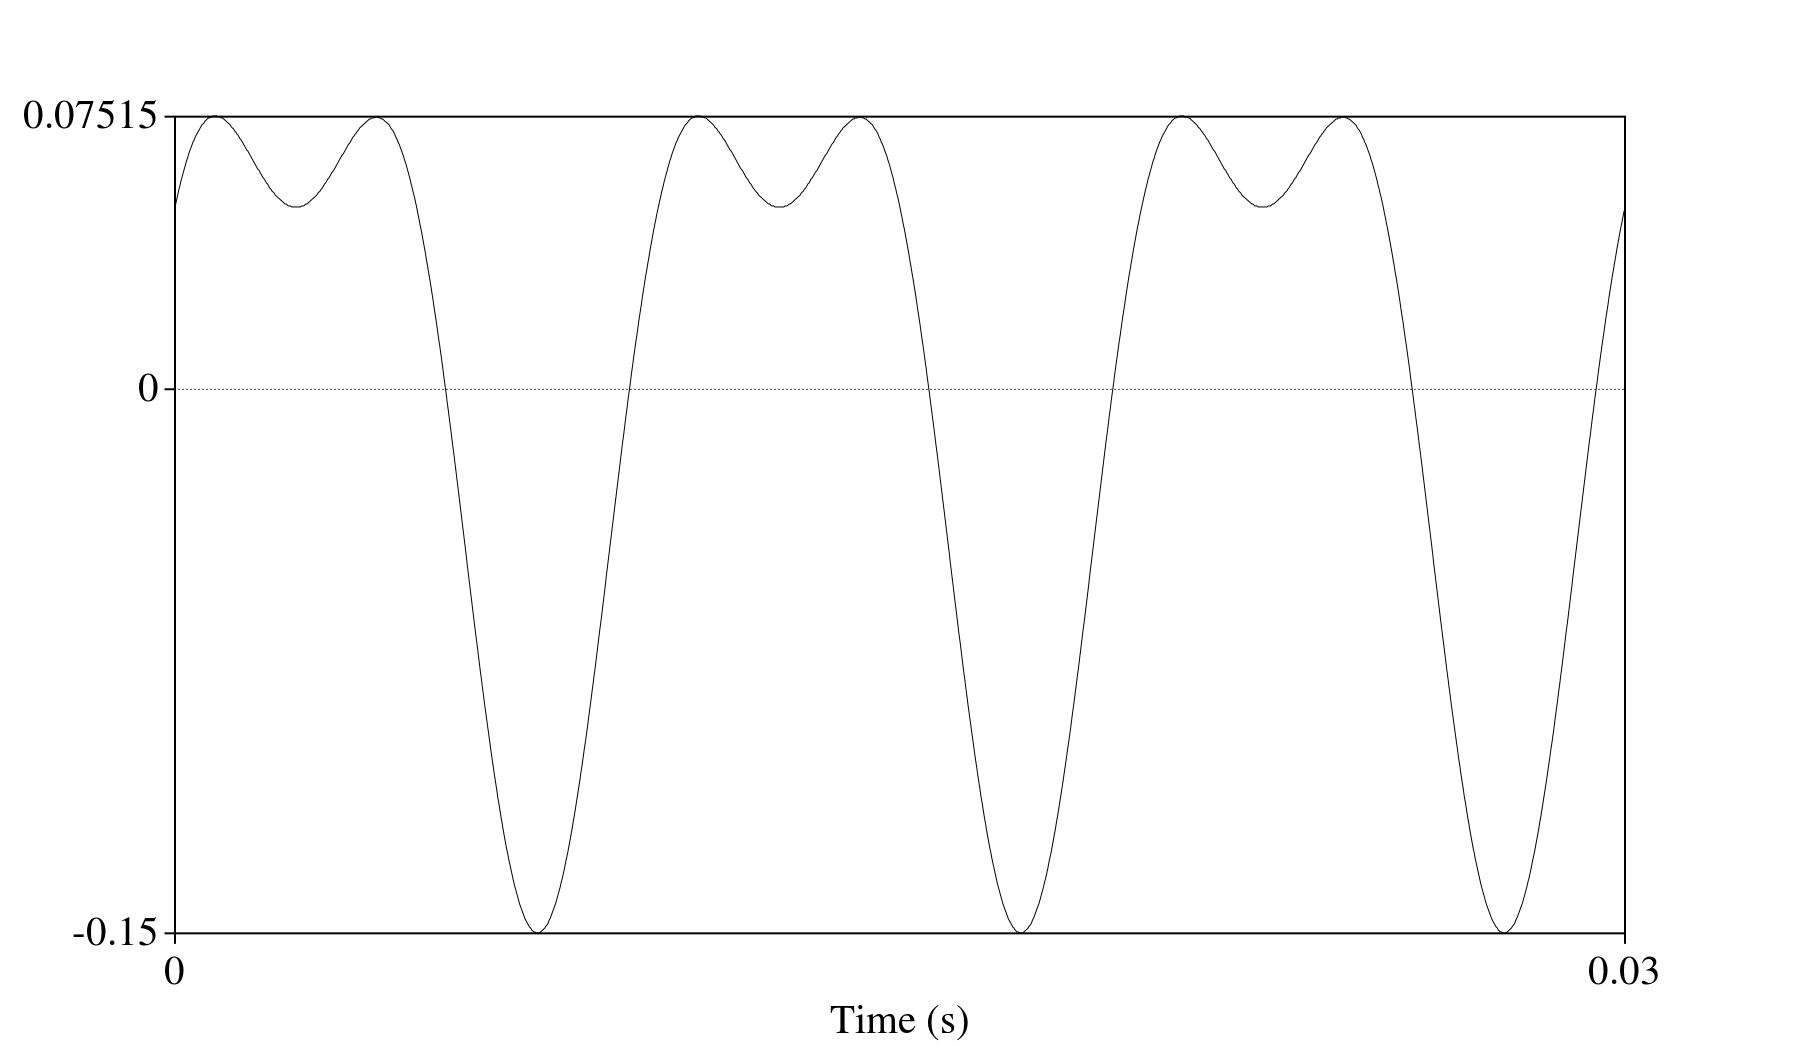
\includegraphics[width=\textwidth]{figure/sound-combined-shifted-phase.png}
  \caption{The sound wave resulting from the combination of the two out of phase waves in Fig. \ref{fig:wave-out-of-phase}.}
  \label{fig:sound-combined-shifted-phase}
\end{subfigure}
\end{center}
\caption{Demonstration of the combination of the waves in Fig. \ref{fig:sound-wave-addition}, where the phase of the 200 Hz wave in Fig. \ref{fig:sound-wave-B} was shifted slightly (cf. Fig. \ref{fig:wave-addition-200hz-shifted})}
\label{fig:sound-shifted-phase}
\end{figure}



\subsection{Difficulties of Speech in Noise}\label{sec:snr-difficult}

Nevertheless, there are still situations in which it is difficult to parse speech in noise.  This is most often due to signals with energy at similar frequencies that overlap.  The greater the amplitude of a signal at frequencies overlapping with those of speech, the more difficult the speech will be to understand.  This can be visualized in the spectrograms of the sentence ``A rich farm is rare in this sandy waste.'' in Figure \ref{fig:signal-SNR-intro}.  As demonstrated before in Figure \ref{fig:signal-SNR-intro-high}, the amplitude, of the noise is well below that of speech, which would likely be easily understand by a listener.  Figure \ref{fig:signal-SNR-intro-low} depicts a much greater noise amplitude level compared to the amplitude level of speech and consequently would likely be more difficult for a listener to understand.

This relationship between speech and any background noise is called the signal to noise ratio (SNR).  A complex signal with a higher signal to noise ratio (cf. Fig \ref{fig:signal-SNR-intro-high}) is generally easier to understand, because the amplitude of the speech (the `signal' of interest) is much greater than that of the noise.  Consequently a lower SNR (cf. Fig. \ref{fig:signal-SNR-intro-low}) results in speech that is more difficult to understand, because the amplitude of the speech is close to - or below - the amplitude of the background noise.  Noise occurring a similar frequency region to the desired speech signal is said to `mask' the speech; this is described in more detail in Chapter \ref{chapter3} (\cite{mattys:12}).

This poses a problem for human listeners in very low SNR environments, but generally is more difficult to deal with for automatic speech recognition (ASR) systems, since the computational system does not contain a highly-skilled, built-in auditory cortex.  There are a number of ways which have been proposed to deal with noise in a speech signal, both for human and automatic speech recognition.  These will be discussed further in Chapters \ref{chapter3} and \ref{chapter4}.

\section{Overview of Dissertation}\label{ch1:diss-overview}

This report aims to explore a novel method of human speech perception and automatic speech recognition (ASR) in noisy environments.  The method proposes that speech be recorded from the inside of the ear canal of the speaker, slightly transformed, and sent to the human listener or the computer receiver for recognition.  Collecting speech from the ear allows for usage of the human skull and adjacent tissues to passively filter out the noisy environment, leaving only - or mostly - the human speech carrying the intended message.  
	
The intention of this study is to determine a) if recording human speech from the inside of the ear canal can significantly reduce background noise in a signal, b) if intelligible speech, suitable for communication, can be collected from the inside of the ear canal, c) if humans find speech recorded from the ear canal more intelligible than speech in noisy conditions, and finally d) if ASR systems are able to recognize speech recorded in the ear canal with greater accuracy than speech recorded in noise.
	
Since at the time, there was no established corpus of data that contains speech recorded from the inside of the ear canal together with speech simultaneously recorded from the mouth in noisy environments, it was necessary to record sounds from speakers in this environment and create a new corpus.  The theory behind the acoustics of recording speech from the ear canal, as well as the process for developing this corpus are described in Chapter \ref{chapter2}, along with a discussion of the recorded speech.  Chapter \ref{chapter3} will outline a human perception experiment, tasking listeners with the transcription of various sentences of speech recorded both at the mouth in noise, and from a sealed ear canal.  Chapter \ref{chapter4} describes the use of this same speech with an ASR system, and its recognition performance.  Chapter \ref{chapter5} will summarize the previous chapters and engage in an overall discussion of the implications of the results, the limitations of the present experiments and methods, and suggestions for future research direction.


